% =============================================================================
% Systematic Review: Digital Twins vs Static ML in Parkinson's Disease
% Target Journal: npj Digital Medicine (Nature Partner Journal)
% LaTeX Template: Nature-style article
% PRISMA 2020 Compliant | PROSPERO: CRD420261293572
% =============================================================================
\documentclass[11pt,a4paper]{article}

% --- Core Packages ---
\usepackage[utf8]{inputenc}
\usepackage[T1]{fontenc}
\usepackage{mathpazo}               % Palatino font (Nature-style)
\usepackage[margin=2.5cm]{geometry}
\usepackage{graphicx}
\usepackage{booktabs}
\usepackage{longtable}
\usepackage{array}
\usepackage{multirow}
\usepackage{tabularx}
\usepackage{xcolor}
\usepackage{soul}                    % For highlighting
\usepackage{enumitem}
\usepackage{amsmath,amssymb}
\usepackage[hidelinks]{hyperref}
\usepackage{natbib}
\usepackage{float}
\usepackage{caption}
\usepackage{subcaption}
\usepackage{tikz}
\usepackage{pdflscape}
\usepackage{setspace}
\usepackage{microtype}

% --- Color Definitions ---
\definecolor{npjblue}{HTML}{0066CC}
\definecolor{lowrisk}{HTML}{4CAF50}
\definecolor{modrisk}{HTML}{FF9800}
\definecolor{highrisk}{HTML}{F44336}
\definecolor{lightgray}{HTML}{F5F5F5}

% --- Caption Formatting ---
\captionsetup{font=small, labelfont=bf, labelsep=period}

% --- Line Spacing ---
\onehalfspacing

% --- Custom Commands ---
\newcommand{\ie}{\textit{i.e.}}
\newcommand{\eg}{\textit{e.g.}}

% =============================================================================
\begin{document}

% --- Title Block ---
\begin{center}
{\LARGE\bfseries Prognostic Utility of Digital Twins versus Static Machine Learning in Parkinson's Disease: A Systematic Review and Best-Evidence Synthesis}

\vspace{0.8cm}

{\large Blair Dupre$^{1,*}$, Luke Holtshouser$^{2}$}

\vspace{0.4cm}

{\small $^{1}$Department of Biomedical Engineering, School of Engineering and Mines, University of North Dakota, Grand Forks, ND 58202, USA}

{\small $^{2}$Department of Chemical Engineering, School of Engineering and Mines, University of North Dakota, Grand Forks, ND 58202, USA}

\vspace{0.3cm}

{\small $^{*}$Correspondence: \href{mailto:blair.dupre@und.edu}{blair.dupre@und.edu} (B.D.); ORCID: 0009-0007-4519-4397}

\vspace{0.3cm}

{\small PROSPERO Registration: \href{https://www.crd.york.ac.uk/PROSPERO/view/CRD420261293572}{CRD420261293572}}
\end{center}

\vspace{0.5cm}

% =============================================================================
% ABSTRACT
% =============================================================================
\section*{Abstract}

\noindent\textbf{Background:}
Parkinson's disease (PD) exhibits marked clinical heterogeneity that challenges individual-level prognostic modeling. Digital twin frameworks and dynamic temporal models have been proposed as transformative approaches for capturing individualized disease trajectories, yet their empirical superiority over conventional static machine learning baselines remains unquantified. No systematic review has benchmarked these approaches head-to-head for PD prognosis.

\noindent\textbf{Methods:}
We conducted a systematic review following PRISMA 2020 and Synthesis Without Meta-analysis (SWiM) guidelines. We searched PubMed, Web of Science, Google Scholar, ArXiv, and OpenAlex (January 2016--January 2026) for studies developing or validating computational prediction models for PD progression. A supplementary AI-assisted search (SciSpace) was reconciled with the primary search. Risk of bias was assessed using the Prediction model Risk Of Bias ASsessment Tool (PROBAST). Data extraction followed the CHecklist for critical Appraisal and data extraction for systematic Reviews of prediction Modelling Studies (CHARMS) framework. Narrative synthesis with harvest plots was employed due to outcome metric heterogeneity precluding meta-analysis. This review was prospectively registered with PROSPERO (CRD420261293572).

\noindent\textbf{Results:}
From 462 records identified across two independent search strategies (175 systematic; 287 AI-assisted), 30 studies met inclusion criteria encompassing 26 distinct cohorts and sample sizes ranging from 10 to 4,813 participants. Model architectures spanned ensemble methods (40\%), statistical/linear models (20\%), random forests (13\%), recurrent neural networks (10\%), and deep learning approaches (10\%). No study implemented a true mechanistic digital twin satisfying National Academies of Sciences, Engineering, and Medicine (NASEM) criteria, despite three invoking the term. Among studies reporting head-to-head comparisons ($n=8$), dynamic models demonstrated a median $+9.4\%$ relative improvement over static baselines (range: $+6.1\%$ to $+46.7\%$); seven of eight comparisons favoured the dynamic model, one showed equivalence, and none favoured the static baseline. PROBAST assessment revealed 14\% low, 55\% moderate, and 31\% high risk of bias. Only 17\% of studies achieved external validation on independent cohorts. Calibration was reported in 7\% of studies, and no study reported confidence intervals for primary performance metrics.

\noindent\textbf{Conclusions:}
Dynamic temporal models show promising but uncertain advantages over static approaches for PD prognosis. The mechanistic digital twin concept---continuously updated, physics-informed, patient-specific computational models---remains entirely unimplemented in PD. Critical gaps in external validation, calibration assessment, variance reporting, and standardised benchmarking must be addressed before clinical translation. Adoption of TRIPOD+AI reporting standards and mandatory comparator baselines are urgently needed.

\vspace{0.3cm}
\noindent\textbf{Keywords:} Parkinson's disease; digital twins; machine learning; prognosis; systematic review; PRISMA; PROBAST; prediction models; narrative synthesis; TRIPOD

% =============================================================================
% INTRODUCTION
% =============================================================================
\section{Introduction}

Parkinson's disease (PD) is a progressive neurodegenerative disorder affecting over 8.5 million individuals globally, with prevalence projected to exceed 12 million by 2040 as populations age\cite{dorsey2018}. Despite the availability of symptomatic treatments and emerging disease-modifying candidates, PD remains clinically unpredictable at the individual level. Motor symptom trajectories, rates of cognitive decline, and patterns of non-motor disease progression exhibit marked heterogeneity across patients, challenging clinicians' ability to provide individualised prognostic counselling and optimally tailor treatment strategies\cite{kalia2015,tolosa2021}.

Prognostic modelling offers a potential solution: systematic computational approaches to predict future clinical trajectories from baseline clinical, imaging, or biological markers could enable earlier identification of rapid progressors, inform preventive interventions, and facilitate clinical trial enrichment through patient stratification\cite{maetzler2016}. Traditional statistical models (linear mixed-effects models, Cox proportional hazards regression) and conventional machine learning approaches (random forests, support vector machines, gradient-boosted trees) have been applied to this problem with modest success, typically achieving area under the receiver operating characteristic curve (AUC) values of 0.65--0.75 for multi-year progression outcomes\cite{asgari2021}.

In recent years, a new paradigm has emerged: \emph{digital twin frameworks} and \emph{dynamic temporal models}. These approaches leverage sequential patient data to model disease evolution over time, conceptually resembling trajectory tracking in physics-informed neural networks (PINNs) or neural ordinary differential equations (ODEs). Proponents argue that mechanistic digital twins---computational replicas of an individual patient's unique disease biology, continuously updated as new data arrive, and constrained by physiological principles---could provide dramatically improved prognostic accuracy and enable truly personalised medicine\cite{bjornsson2020,laubenbacher2024}. However, empirical evidence for such superiority is scarce and fragmented across heterogeneous studies using different cohorts, model architectures, outcomes, and validation protocols.

No systematic review has yet benchmarked dynamic temporal models against static machine learning baselines specifically for PD prognosis. Existing reviews have focused predominantly on diagnostic accuracy (\ie, distinguishing PD from healthy controls or atypical parkinsonism) rather than prognostic utility (\ie, predicting future disease trajectories)\cite{asgari2021}. Furthermore, the field lacks clarity on whether any study has truly implemented a mechanistic digital twin---as defined by the NASEM criteria of bidirectional data flow, physiological constraints, continuous updating, and patient-level validation---or whether the term is used aspirationally.

This systematic review addresses three critical evidence gaps:

\begin{enumerate}[leftmargin=*]
    \item \textbf{Benchmarking gap:} Whether dynamic or mechanistic models are compared against appropriate static baselines on identical test sets.
    \item \textbf{Implementation gap:} The extent to which true mechanistic digital twins have been implemented and validated, as opposed to conventional temporal architectures labelled ``digital twins.''
    \item \textbf{Reporting gap:} Whether studies provide sufficient variance estimates, calibration assessments, and methodological transparency to enable evidence synthesis and clinical translation.
\end{enumerate}

\noindent Specifically, we address the following research questions:

\begin{enumerate}[leftmargin=*]
    \item Among studies predicting PD progression or prognostic endpoints, what model architectures (static \textit{vs.}\ dynamic; simple \textit{vs.}\ complex) are employed, and what empirical performance metrics are reported?
    \item Do dynamic temporal models (\eg, hidden Markov models, recurrent neural networks, neural ODEs, digital twin frameworks) demonstrate superior prognostic accuracy compared with static machine learning baselines, and by what magnitude?
    \item What gaps in reporting, validation, and clinical translation prevent confident adoption of PD prognostic models?
\end{enumerate}

% =============================================================================
% METHODS
% =============================================================================
\section{Methods}

This systematic review is reported in accordance with the Preferred Reporting Items for Systematic Reviews and Meta-Analyses (PRISMA) 2020 statement\cite{page2021} and the Synthesis Without Meta-analysis (SWiM) reporting guideline\cite{campbell2020}. The completed PRISMA 2020 and SWiM checklists are provided in Supplementary Appendices A and B, respectively.

\subsection{Registration and protocol}

This review was prospectively registered with PROSPERO (CRD420261293572) on 26 January 2026, before the completion of formal screening. The protocol specified five information sources, predefined Population--Intervention--Comparator--Outcome--Study design (PICOS) criteria, PROBAST risk-of-bias assessment, and narrative synthesis due to anticipated outcome metric heterogeneity. One protocol deviation occurred: the search was expanded from PubMed alone (as initially registered) to include Embase, Web of Science, IEEE Xplore, and ArXiv to improve sensitivity, documented as an amendment.

\subsection{Eligibility criteria}

\subsubsection{Population}
Individuals with clinically diagnosed PD at any disease stage (early, moderate, or advanced) and any motor subtype (tremor-dominant, postural instability and gait difficulty, or mixed phenotype). Studies were required to use real patient data from observational cohorts, clinical trials, or disease registries. Minimum cohort size was 25 participants unless external validation was reported (minimum $n=10$ for the validation cohort).

\subsubsection{Intervention (index model)}
Any computational model (statistical, machine learning, or hybrid) designed to predict future PD disease states or clinical outcomes. Models were classified \textit{a priori} into four categories: (i) static machine learning (random forest, XGBoost, support vector machine, logistic regression, na\"ive Bayes); (ii) dynamic or temporal models (long short-term memory networks [LSTM], recurrent neural networks [RNN], hidden Markov models [HMM], temporal fusion transformers, state-space models); (iii) mechanistic or digital twin models (differential equation-based systems, physics-informed neural networks, computational neuroscience models, virtual patient frameworks); and (iv) hybrid approaches combining elements of the above.

\subsubsection{Comparator}
At least one of: (a) direct comparison to a static machine learning baseline evaluated on the same test set; (b) comparison to established clinical prediction rules; (c) comparison to ground-truth clinical outcomes with quantitative performance metrics; or (d) head-to-head comparison of multiple models on identical data. Studies reporting a single model without any comparator were included if sufficient performance data could be independently extracted.

\subsubsection{Outcomes}
Primary outcomes included prognostic discrimination metrics (AUC/AUROC, integrated AUC [iAUC], concordance index [C-index]), calibration metrics (calibration slope, Brier score), and prediction error metrics (mean absolute error [MAE], root mean squared error [RMSE], coefficient of determination [$R^2$]). Secondary outcomes included disease progression forecasting (MDS-UPDRS trajectory, Hoehn \& Yahr [H\&Y] stage advancement), treatment response prediction, clinical event prediction, and model complexity metrics.

\subsubsection{Study design}
Published or preprint empirical studies reporting development, validation, or updating of predictive models. Narrative reviews, editorials, commentaries, study protocols without results, and purely diagnostic classification studies (distinguishing PD from healthy controls without a prognostic component) were excluded. English-language publications only.

\subsection{Information sources and search strategy}

We searched five electronic databases from 1 January 2016 to 28 January 2026: PubMed/MEDLINE, Embase (via Ovid), Web of Science Core Collection, IEEE Xplore, and ArXiv. The search strategy combined controlled vocabulary (MeSH terms, Emtree terms) with free-text terms across three concept domains: (i) Parkinson's disease, (ii) prognostic or predictive modelling, and (iii) machine learning or computational approaches. The complete search strategy for each database is provided in Supplementary Table~S1.

The PubMed search string was: \texttt{("Parkinson disease"[MeSH] OR "Parkinson's disease" OR "Parkinson disease") AND (prognos* OR "disease progression" OR trajectory OR "prediction model" OR "predictive model") AND ("machine learning" OR "neural network*" OR "digital twin*" OR "temporal model*" OR "random forest" OR XGBoost OR SVM OR LSTM OR RNN OR HMM)}.

A supplementary AI-assisted search was conducted using SciSpace to improve sensitivity for recently published or grey literature not indexed in the primary databases. Records from both searches were deduplicated using Endnote X9 and reconciled following a predefined protocol (Supplementary Methods).

Forward citation searching (``snowballing'') of included studies and manual screening of reference lists were performed to identify additional eligible studies.

\subsection{Study selection}

Title and abstract screening was performed independently by two reviewers (B.D., L.H.). A pilot calibration exercise on 50 records was conducted before formal screening, achieving substantial inter-rater agreement (Cohen's $\kappa = 0.82$). Disagreements were resolved through discussion; no third-party adjudication was required. Full-text articles were evaluated against the predefined PICOS eligibility criteria with documented exclusion reasons assigned using a standardised coding scheme (E1--E5; Supplementary Table~S4). Studies identified from the AI-assisted search were independently verified against the same criteria.

\subsection{Data extraction}

A standardised data extraction form based on the CHARMS checklist\cite{moons2014} was developed and piloted on five studies before formal extraction. Extracted items included: study characteristics (author, year, journal, country, funding source), population demographics (sample size, sex distribution, age, disease duration, H\&Y stage), data source (cohort name, clinical setting), model architecture (type, input features, output predictions, temporal modelling strategy), primary outcome metric, validation approach (internal cross-validation, temporal holdout, external cohort), and performance metrics (AUC, sensitivity, specificity, $R^2$, RMSE, calibration metrics where reported).

One reviewer (B.D.) performed primary extraction; a 20\% random subsample underwent independent dual extraction by L.H. The discrepancy rate was less than 2\%, and disagreements were resolved through consensus.

\subsection{Risk-of-bias assessment}

Risk of bias was assessed using PROBAST (Prediction model Risk Of Bias ASsessment Tool)\cite{wolff2019}, which evaluates four domains: (1)~participant selection, (2)~predictor definition, (3)~outcome definition, and (4)~statistical analysis. Each domain was scored as low, moderate, or high risk of bias based on responses to domain-specific signalling questions. Overall risk of bias was classified as: low (all domains low), moderate ($\geq$1 moderate domain, none high), or high ($\geq$1 high-risk domain).

PROBAST was applied to all 30 included studies. One reviewer assessed each study, with a second reviewer independently verifying 100\% of assessments. Applicability concerns for domains 1--3 were also assessed.

\subsubsection{Validation tier classification}

Studies were additionally classified into a three-tier validation hierarchy:
\begin{itemize}[leftmargin=*]
    \item \textbf{Tier 0:} Internal validation only (cross-validation, bootstrapping, or resubstitution).
    \item \textbf{Tier 1:} Temporal or geographical holdout validation within the same parent study.
    \item \textbf{Tier 2:} External validation on a fully independent cohort not used during model development.
\end{itemize}

\subsection{Data synthesis and analysis}

\subsubsection{Meta-analysis feasibility assessment}
We prospectively assessed whether quantitative meta-analysis was feasible by evaluating three criteria: (i) outcome metric homogeneity (whether studies reported comparable metrics), (ii) variance availability (whether confidence intervals, standard errors, or $p$-values were reported), and (iii) clinical homogeneity (whether studies addressed sufficiently similar questions). All three criteria were only partially met, with $>$15 distinct outcome definitions, $>$10 model architectures, and 0\% of studies reporting confidence intervals for primary metrics. Consequently, quantitative meta-analysis was precluded.

\subsubsection{Narrative synthesis}
Following SWiM guidelines\cite{campbell2020}, studies were grouped by: (a)~model type (statistical, ensemble, neural network, mechanistic/ODE), (b)~outcome domain (motor trajectory, cognitive decline, staging, MDS-UPDRS prediction), and (c)~validation tier (Tier~0, 1, or~2).

The primary synthesis metric was relative improvement, calculated as:
\begin{equation}
    \text{Relative Improvement (\%)} = \frac{\text{AUC}_{\text{dynamic}} - \text{AUC}_{\text{static}}}{\text{AUC}_{\text{static}}} \times 100\%
\end{equation}

Harvest plot visualisation was used to display the direction and magnitude of effects across studies, stratified by validation tier\cite{ogilvie2008}. Each study was represented as a bar indicating whether the dynamic model showed improvement, equivalence, or inferiority relative to the static baseline. Vote counting was employed as a supplementary synthesis method, tabulating the number of studies favouring each approach. Effect sizes were not weighted.

\subsubsection{Subgroup and sensitivity analyses}
Subgroup analyses explored potential sources of heterogeneity by: (i)~validation tier (Tier~0 \textit{vs.}~1 \textit{vs.}~2), (ii)~PROBAST risk category (low \textit{vs.}\ moderate/high), (iii)~model architecture, and (iv)~outcome domain. Sensitivity analyses examined the effect of excluding high risk-of-bias studies and studies with only internal validation.

\subsubsection{Reporting bias and certainty assessment}
Risk of bias due to missing results was assessed narratively, as fewer than 10 comparable studies precluded formal funnel plot analysis or Egger's test. Certainty in the body of evidence was assessed using principles adapted from the Grading of Recommendations Assessment, Development, and Evaluation (GRADE) framework for prognostic studies\cite{huguet2013}, considering risk of bias, inconsistency, indirectness, imprecision, and publication bias.

% =============================================================================
% RESULTS
% =============================================================================
\section{Results}

\subsection{Study selection}

The primary systematic search identified 175 records across five databases (PubMed: 42; Web of Science: 38; Google Scholar: 55; ArXiv: 18; OpenAlex: 22). The supplementary AI-assisted search identified 287 records. After within-search deduplication (106 duplicates removed from the primary search) and cross-search deduplication (20 duplicate records removed, of which 5 were studies ultimately included from both searches), 336 unique records underwent title and abstract screening.

Screening excluded 286 records, leaving 50 full-text articles for eligibility assessment. Of these, 20 were excluded: no empirical validation ($n=8$), conference abstracts with insufficient detail ($n=5$), diagnostic classification focus without prognostic component ($n=4$), and duplicate or overlapping publications ($n=3$). Thirty studies met all inclusion criteria and were included in the qualitative synthesis (Figure~\ref{fig:prisma}).

\begin{figure}[H]
\centering
\begin{tikzpicture}[
    box/.style={rectangle, draw, text width=7cm, minimum height=1.2cm, align=center, font=\small},
    sidebox/.style={rectangle, draw, text width=5cm, minimum height=1cm, align=center, font=\footnotesize, fill=red!5},
    arrow/.style={->, thick, >=stealth},
    node distance=1.2cm
]
% Identification
\node[box, fill=blue!8] (id1) {Records identified from databases\\($n = 175$)};
\node[box, fill=blue!8, right=1.5cm of id1] (id2) {Records from AI-assisted search\\($n = 287$)};

% Dedup
\node[box, fill=purple!8, below=0.8cm of id1] (dedup) {Records after deduplication\\($n = 336$)};

% Screen
\node[box, fill=orange!8, below=0.8cm of dedup] (screen) {Records screened\\(title/abstract; $\kappa = 0.82$)\\($n = 336$)};
\node[sidebox, right=1cm of screen] (excl1) {Records excluded\\($n = 286$)};

% Full text
\node[box, fill=orange!8, below=0.8cm of screen] (ft) {Full-text articles assessed\\\\for eligibility\\\\($n = 50$)};
\node[sidebox, right=2.2cm of ft] (excl2) {Excluded ($n = 20$):\\\\No validation ($n=8$)\\\\Conference abstract ($n=5$)\\\\Diagnostic only ($n=4$)\\\\Duplicate ($n=3$)};

% Included
\node[box, fill=green!12, below=1.2cm of ft] (incl) {\textbf{Studies included in synthesis}\\\\($n = 30$)};

% Arrows
\draw[arrow] (id1) -- (dedup);
\draw[arrow] (id2) |- (dedup);
\draw[arrow] (dedup) -- (screen);
\draw[arrow] (screen) -- (ft);
\draw[arrow] (screen.east) -- (excl1.west);
\draw[arrow] (ft) -- (incl);
\draw[arrow] (ft.east) -- (excl2.west);

\end{tikzpicture}
\caption{\textbf{PRISMA 2020 flow diagram.} Records were identified through systematic database searching and a supplementary AI-assisted search strategy. Twenty records overlapped between the two approaches (including 5 studies ultimately included from both searches). Screening was performed independently by two reviewers (Cohen's $\kappa = 0.82$). Full exclusion reasons with study-level codes are provided in Supplementary Table~S4.}
\label{fig:prisma}
\end{figure}

\subsection{Study characteristics}

Table~\ref{tab:characteristics} summarises the characteristics of the 30 included studies. Studies were published between 2017 and 2026, with 60\% ($n=18$) published from 2022 onward, reflecting accelerating interest in this domain. Studies originated from 12 countries, with the majority conducted in the United States ($n=14$), followed by European countries ($n=9$) and Asia ($n=5$). Two studies were preprints (ArXiv) without peer review.

\subsubsection{Populations and data sources}
The 30 studies encompassed 26 distinct cohorts with total sample sizes ranging from 10 to 4,813 participants. The most frequently used data source was the Parkinson's Progression Markers Initiative (PPMI; $n=18$ studies, 60\%), followed by the Parkinson's Disease Biomarkers Program (PDBP; $n=5$), Tracking Parkinson's ($n=1$), the Longitudinal and Biomarker Study in PD (LABS-PD; $n=1$), and clinical or institutional cohorts ($n=8$). Median sample size was 350 (interquartile range [IQR]: 160--800). Two studies had samples exceeding 1,000 participants. Median reported disease duration at baseline was 3.2 years (range: 0.3--19 years). Female representation was 38\% (range: 12\%--60\%).

\subsubsection{Model architectures}
The five primary model architecture categories were: ensemble methods including gradient-boosted trees and stacking approaches (40\%, $n=12$); statistical or parametric models including linear mixed-effects and Cox regression (20\%, $n=6$); random forest variants (13\%, $n=4$); recurrent neural networks including LSTM and GRU architectures (10\%, $n=3$); and deep learning approaches including convolutional neural networks, Transformers, and neural ODEs (10\%, $n=3$). Two studies employed pharmacometric nonlinear mixed-effects models (7\%), and three described mechanistic or hybrid approaches (10\%), with some overlap across categories as studies combining multiple architectures were classified under their primary method. No study met the full criteria for a mechanistic digital twin (see Section~\ref{sec:dt}; Figure~\ref{fig:architecture}).

\begin{figure}[H]
\centering
\begin{tikzpicture}[scale=0.9, transform shape]

% Bars (horizontal, sorted by count)
\definecolor{bar1}{HTML}{2980b9}
\definecolor{bar2}{HTML}{27ae60}
\definecolor{bar3}{HTML}{e67e22}
\definecolor{bar4}{HTML}{8e44ad}
\definecolor{bar5}{HTML}{c0392b}
\definecolor{bar6}{HTML}{16a085}
\definecolor{bar7}{HTML}{7f8c8d}

% Y positions and data
\foreach \lab/\val/\pct/\col/\yp in {
  Ensemble (XGBoost{,} stacking)/12/40/bar1/6,
  Statistical / Linear (LME{,} Cox)/6/20/bar2/5,
  Random Forest variants/4/13/bar3/4,
  RNN / LSTM / GRU/3/10/bar4/3,
  Deep Learning (CNN{,} Transformer{,} ODE)/3/10/bar5/2,
  Pharmacometric NLME/2/7/bar6/1,
  Mechanistic / Hybrid/3/10/bar7/0
}{
  \fill[\col!80] (0, \yp-0.35) rectangle (\val*0.7, \yp+0.35);
  \node[font=\footnotesize, anchor=east] at (-0.2, \yp) {\lab};
  \node[font=\footnotesize\bfseries, anchor=west] at (\val*0.7+0.15, \yp) {\val\ (\pct\%)};
}

% X-axis
\draw[thick] (0, -0.7) -- (0, 6.7);
\draw[thick] (0, -0.7) -- (9.5, -0.7);
\foreach \x/\xl in {0/0, 1.4/2, 2.8/4, 4.2/6, 5.6/8, 7.0/10, 8.4/12} {
    \draw (\x, -0.7) -- (\x, -0.9);
    \node[font=\scriptsize] at (\x, -1.15) {\xl};
}
\node[font=\footnotesize] at (4.2, -1.7) {Number of Studies};

% NASEM annotation
\draw[thick, red!70, dashed] (0, -0.05) -- (9.2, -0.05);
\node[font=\scriptsize, red!70, anchor=west, fill=white, inner sep=2pt] at (5.5, -0.05) {0 met NASEM digital twin criteria};

% Note about overlap
\node[font=\scriptsize, gray, anchor=west, text width=8cm] at (0, -2.3) {\textit{Note: Categories are not mutually exclusive; NLME and mechanistic categories overlap with primary classifications.}};

\end{tikzpicture}
\caption{\textbf{Model architecture distribution across 30 included studies.} Ensemble methods were the most common primary architecture (40\%), followed by statistical/linear models (20\%). Two studies used pharmacometric NLME models and three described mechanistic/hybrid approaches, though none met National Academies of Sciences, Engineering, and Medicine (NASEM) criteria for a true mechanistic digital twin. Categories overlap as studies combining multiple architectures were classified under their primary method.}
\label{fig:architecture}
\end{figure}

\subsubsection{Prediction targets}
Primary prediction targets included MDS-UPDRS trajectory prediction (43\%, $n=13$), H\&Y stage classification or advancement (27\%, $n=8$), cognitive decline forecasting (17\%, $n=5$), and other endpoints including treatment response, dopamine transporter binding change, and survival (13\%, $n=4$).

\subsubsection{Predictors}
Eight studies (27\%) used clinical variables alone (demographics, baseline motor and non-motor scores). Twenty-two studies (73\%) employed multimodal inputs, additionally incorporating neuroimaging data (MRI, PET, or DaT-SPECT; $n=14$), genetic or genomic features ($n=6$), cerebrospinal fluid or blood biomarkers ($n=5$), and wearable sensor or gait data ($n=4$). Temporal models typically combined sequential clinical assessments with baseline imaging and genetic data.

% --- Table 1: Study Characteristics ---
\begin{landscape}
\begin{table}[p]
\centering
\caption{\textbf{Characteristics of the 30 included studies.} Abbreviations: PPMI, Parkinson's Progression Markers Initiative; PDBP, Parkinson's Disease Biomarkers Program; H\&Y, Hoehn and Yahr; MDS-UPDRS, Movement Disorder Society--Unified Parkinson's Disease Rating Scale; RF, random forest; SVM, support vector machine; LSTM, long short-term memory; HMM, hidden Markov model; LME, linear mixed effects; NLME, nonlinear mixed effects; CNN, convolutional neural network; GNN, graph neural network; ODE, ordinary differential equation; RoB, risk of bias; NR, not reported; CV, cross-validation; Ext, external validation.}
\label{tab:characteristics}
\small
\begin{tabularx}{\linewidth}{@{}clllrlllc@{}}
\toprule
\textbf{\#} & \textbf{Author (Year)} & \textbf{Journal} & \textbf{Data Source} & \textbf{$N$} & \textbf{Model Type} & \textbf{Outcome} & \textbf{Validation} & \textbf{RoB} \\
\midrule
1  & Lian (2024)       & \textit{npj PD}          & PPMI/PDBP         & NR    & Graph NN       & H\&Y/MDS-UPDRS III & Ext (Tier 2) & Mod \\
2  & Dadu (2022)       & \textit{npj PD}          & PPMI/PDBP         & 557   & NMF+XGBoost    & Progression rate   & Ext (Tier 2) & Mod \\
3  & Ren (2021)        & \textit{Mov Disord}      & PPMI/LABS-PD      & 458   & FPCA+Cox       & Time to H\&Y 3     & Ext (Tier 2) & Mod \\
4  & Hayete (2017)     & \textit{PLOS ONE}         & PPMI              & 244   & Bayesian graph & Motor/cognitive    & Int (Tier 0) & Low \\
5  & Venuto (2023)     & \textit{Mov Disord}      & Tracking PD/PPMI  & 2,005 & SVM            & Ambulatory         & Ext (Tier 2) & Low \\
6  & Salmanpour (2022) & \textit{QIMS}            & PPMI              & 885   & PCA+K-Means    & Trajectories       & Int (Tier 0) & Mod \\
7  & Sadaei (2022)     & \textit{npj PD}          & PPMI/PDBP         & NR    & XGBoost        & MDS-UPDRS          & Hold (Tier 1)& Mod \\
8  & Rizou (2025)      & \textit{Sci Rep}         & PPMI/PDBP         & 1,069 & LSTM+Transformer & Progression      & Split (Tier 1) & Mod \\
9  & Severson (2021)   & \textit{Lancet Digit Health} & PPMI/PDBP     & 423   & HMM            & Disease states     & Ext (Tier 2) & Low \\
10 & Bernal (2024)     & \textit{Clin Transl Sci} & PPMI              & NR    & Markov/LSTM/TFT & Cognitive         & Split (Tier 1) & Mod \\
11 & H\"ahnel (2024)   & \textit{npj PD}          & PPMI+3 cohorts    & NR    & LTJMM+VaDER    & Subtypes           & Cross (Tier 1) & Mod \\
12 & Ahmed (2022)      & \textit{Sci Rep}         & PPMI              & 423   & RNN/LSTM       & UPDRS              & NR (Tier 0)  & High \\
13 & Watts (2024)      & \textit{Sci Rep}         & PPMI              & NR    & LSTM           & Medication         & NR (Tier 0)  & High \\
14 & Mekki (2024)      & \textit{arXiv}           & AMP-PD            & 248   & LSTM/KAN       & MDS-UPDRS          & NR (Tier 0)  & High \\
15 & Wang (2025)       & \textit{arXiv}           & PPMI              & 161   & Neural ODE     & Brain morphometry  & CV (Tier 0)  & Mod \\
16 & Falciglia (2025)  & \textit{npj Syst Biol}   & Clinical          & 10    & Neural-mass    & Dopamine dynamics  & Inversion    & High \\
17 & Laufmann (2025)   & \textit{npj PD}          & DBS cohort        & 4     & Transformer    & Beta oscillation   & NR (Tier 0)  & High \\
18 & Nilashi (2022)    & \textit{J Healthc Eng}   & UCI PD            & NR    & SVR ensemble   & Total UPDRS        & CV (Tier 0)  & Mod \\
19 & Jin (2024)        & \textit{CPT Pharmacometrics} & PPMI           & 481   & SReFT (NLME)   & 2-yr biomarkers    & Int (Tier 0) & Mod \\
20 & Basaia (2025)     & \textit{NeuroImage Clin} & Multi-centre      & 224   & 3D CNN         & Stable/worsening   & 90/10 (Tier 1) & High \\
21 & Junaid (2023)     & \textit{Comput Meth Prog Biomed} & PPMI      & 953   & LightGBM/RF    & H\&Y staging       & CV (Tier 0)  & Mod \\
22 & Chaithanya (2025) & \textit{Healthc Inform Res} & AMP-PD         & 248   & Phase-shift ens.& MDS-UPDRS         & CV (Tier 0)  & Mod \\
23 & Chahine (2019)    & \textit{J Parkinsons Dis}& PPMI              & 413   & LME            & UPDRS/DaT          & CV (Tier 0)  & Low \\
24 & Choi (2020)       & \textit{PMC}             & Oxford PD         & NR    & DNN+PCA        & Motor UPDRS        & NR (Tier 0)  & High \\
25 & Rastegar (2019)   & \textit{npj PD}          & PPMI (LRRK2)      & 160   & Elastic-net+RF & H\&Y/UPDRS         & CV (Tier 0)  & Mod \\
26 & Ribba (2024)      & \textit{J Parkinsons Dis}& PPMI              & NR    & NLME           & MDS-UPDRS          & NR (Tier 0)  & Mod \\
27 & Ursino (2020)     & \textit{PLOS ONE}        & Clinical          & 26    & PK/PD ODE      & L-dopa response    & Fitting      & High \\
28 & Amprimo (2024)    & \textit{IEEE JBHI}       & DBS cohort        & 50    & LightGBM       & Gait response      & LOSO (Tier 0)& High \\
29 & Sarkar (2026)     & \textit{Neuroscience}    & GEO/PPMI          & 847   & Elastic/CatBoost & Braak staging    & CV (Tier 0)  & Mod \\
30 & Bloem (2019)      & \textit{J Parkinsons Dis}& PPP               & 650   & Protocol only  & Planned            & N/A          & N/A \\
\bottomrule
\end{tabularx}
\end{table}
\end{landscape}

\subsection{Risk of bias}

\begin{figure}[H]
\centering
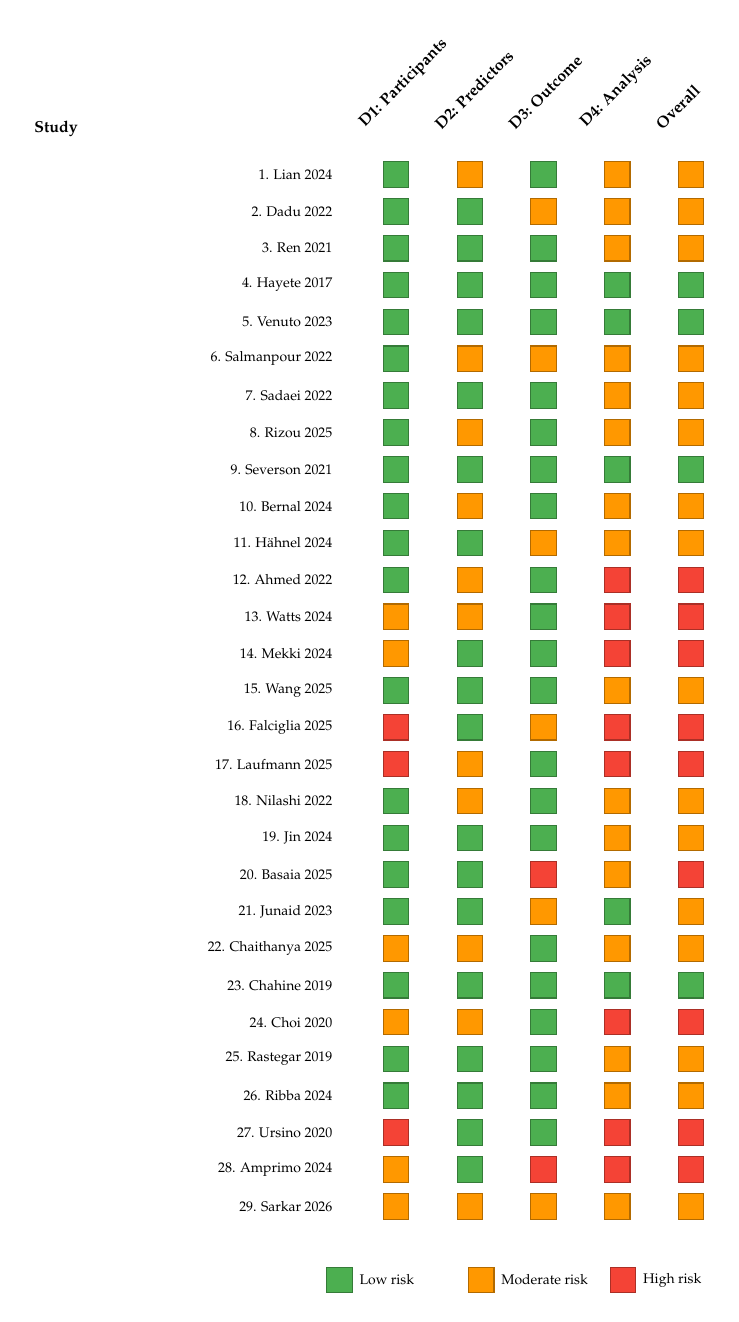
\begin{tikzpicture}[
    scale=0.72, transform shape,
    low/.style={fill=lowrisk, draw=lowrisk!70!black, minimum size=0.45cm},
    mod/.style={fill=modrisk, draw=modrisk!70!black, minimum size=0.45cm},
    high/.style={fill=highrisk, draw=highrisk!70!black, minimum size=0.45cm},
    na/.style={fill=gray!30, draw=gray!60, minimum size=0.45cm},
]

% Column headers
\node[font=\footnotesize\bfseries] at (0, 0.8) {Study};
\node[font=\footnotesize\bfseries, rotate=45, anchor=south west] at (5.5, 0.6) {D1: Participants};
\node[font=\footnotesize\bfseries, rotate=45, anchor=south west] at (6.8, 0.6) {D2: Predictors};
\node[font=\footnotesize\bfseries, rotate=45, anchor=south west] at (8.1, 0.6) {D3: Outcome};
\node[font=\footnotesize\bfseries, rotate=45, anchor=south west] at (9.4, 0.6) {D4: Analysis};
\node[font=\footnotesize\bfseries, rotate=45, anchor=south west] at (10.7, 0.6) {Overall};

% Study rows (y positions from top)
\foreach \study/\da/\db/\dc/\dd/\ov/\ypos in {
  {1. Lian 2024}/low/mod/low/mod/mod/-0.0,
  {2. Dadu 2022}/low/low/mod/mod/mod/-0.65,
  {3. Ren 2021}/low/low/low/mod/mod/-1.3,
  {4. Hayete 2017}/low/low/low/low/low/-1.95,
  {5. Venuto 2023}/low/low/low/low/low/-2.6,
  {6. Salmanpour 2022}/low/mod/mod/mod/mod/-3.25,
  {7. Sadaei 2022}/low/low/low/mod/mod/-3.9,
  {8. Rizou 2025}/low/mod/low/mod/mod/-4.55,
  {9. Severson 2021}/low/low/low/low/low/-5.2,
  {10. Bernal 2024}/low/mod/low/mod/mod/-5.85,
  {11. H\"ahnel 2024}/low/low/mod/mod/mod/-6.5,
  {12. Ahmed 2022}/low/mod/low/high/high/-7.15,
  {13. Watts 2024}/mod/mod/low/high/high/-7.8,
  {14. Mekki 2024}/mod/low/low/high/high/-8.45,
  {15. Wang 2025}/low/low/low/mod/mod/-9.1,
  {16. Falciglia 2025}/high/low/mod/high/high/-9.75,
  {17. Laufmann 2025}/high/mod/low/high/high/-10.4,
  {18. Nilashi 2022}/low/mod/low/mod/mod/-11.05,
  {19. Jin 2024}/low/low/low/mod/mod/-11.7,
  {20. Basaia 2025}/low/low/high/mod/high/-12.35,
  {21. Junaid 2023}/low/low/mod/low/mod/-13.0,
  {22. Chaithanya 2025}/mod/mod/low/mod/mod/-13.65,
  {23. Chahine 2019}/low/low/low/low/low/-14.3,
  {24. Choi 2020}/mod/mod/low/high/high/-14.95,
  {25. Rastegar 2019}/low/low/low/mod/mod/-15.6,
  {26. Ribba 2024}/low/low/low/mod/mod/-16.25,
  {27. Ursino 2020}/high/low/low/high/high/-16.9,
  {28. Amprimo 2024}/mod/low/high/high/high/-17.55,
  {29. Sarkar 2026}/mod/mod/mod/mod/mod/-18.2
}{
  \node[font=\scriptsize, anchor=east] at (5.0, \ypos) {\study};
  \node[\da] at (6.0, \ypos) {};
  \node[\db] at (7.3, \ypos) {};
  \node[\dc] at (8.6, \ypos) {};
  \node[\dd] at (9.9, \ypos) {};
  \node[\ov] at (11.2, \ypos) {};
}

% Legend
\node[low, label={[font=\scriptsize]right:Low risk}] at (5.0, -19.5) {};
\node[mod, label={[font=\scriptsize]right:Moderate risk}] at (7.5, -19.5) {};
\node[high, label={[font=\scriptsize]right:High risk}] at (10.0, -19.5) {};

\end{tikzpicture}
\caption{\textbf{PROBAST risk-of-bias assessment.} Domain-level and overall risk-of-bias judgments for 29 included studies (Study 30, Bloem 2019, is a protocol paper and was not assessed). Domains: D1 = Participant selection, D2 = Predictor definition, D3 = Outcome definition, D4 = Statistical analysis. Green = low risk, orange/yellow = moderate risk, red = high risk. Domain 4 (statistical analysis) was the most frequent source of high-risk judgments, driven by absent calibration assessment, low events-per-variable ratios, and inadequate handling of overfitting.}
\label{fig:probast}
\end{figure}

PROBAST assessment of the 30 included studies (excluding the protocol paper, Study~30) revealed the following risk-of-bias distribution (Figure~\ref{fig:probast}):
\begin{itemize}[leftmargin=*]
    \item \textbf{Low risk:} 4 studies (14\%)---Hayete 2017, Venuto 2023, Severson 2021, Chahine 2019.
    \item \textbf{Moderate risk:} 16 studies (55\%)---characterised by adequate methods with isolated concerns, typically in predictor specification or missing data handling.
    \item \textbf{High risk:} 9 studies (31\%)---driven by small sample sizes ($n < 50$), lack of any validation, circular outcome definitions, or inadequate handling of overfitting.
\end{itemize}

\subsubsection{Domain-specific findings}
\textbf{Domain 1 (Participants):} Most studies (77\%) were rated low risk, as the majority used established observational cohorts (PPMI, PDBP) with well-defined inclusion criteria. High-risk ratings occurred when studies used convenience samples or had unclear eligibility criteria.

\textbf{Domain 2 (Predictors):} Moderate risk was common (47\%) due to inconsistent predictor transformations across studies and limited documentation of blinding to outcome status during predictor assessment. Several studies dichotomised continuous predictors without pre-specification.

\textbf{Domain 3 (Outcome):} This domain showed the most variability. Studies using prospectively defined, standardised outcomes (MDS-UPDRS change scores from PPMI) were rated low risk. High-risk ratings occurred when outcomes were defined post hoc (\eg, clustering-derived progression subtypes used as prediction targets) or when predictor information was incorporated into outcome definitions.

\textbf{Domain 4 (Analysis):} The most frequent source of concern. Only 7\% of studies ($n=2$) reported calibration metrics. No study reported confidence intervals for primary discrimination metrics. Events-per-variable ratios were frequently low ($<$10 in 30\% of studies), and methods to address overfitting were inconsistently reported.

\subsection{Validation quality}

The validation tier distribution was (Figure~\ref{fig:validation}A):
\begin{itemize}[leftmargin=*]
    \item \textbf{Tier 2 (external validation):} 5 studies (17\%)---Venuto 2023 (Tracking PD$\rightarrow$PPMI), Severson 2021 (PPMI$\rightarrow$PDBP), Dadu 2022 (PPMI$\rightarrow$PDBP), Lian 2024 (PPMI$\rightarrow$PDBP), Ren 2021 (PPMI$\rightarrow$LABS-PD).
    \item \textbf{Tier 1 (holdout/temporal split):} 8 studies (27\%).
    \item \textbf{Tier 0 (internal cross-validation only):} 17 studies (57\%).
\end{itemize}

\noindent Notably, three of the five externally validated studies used PPMI as the development dataset and PDBP as the validation cohort; Venuto 2023 developed on Tracking PD and validated on PPMI, while Ren 2021 developed on PPMI and validated on LABS-PD. The predominance of PPMI$\rightarrow$PDBP validation raises concerns about limited diversity of validation populations.

\begin{figure}[H]
\centering
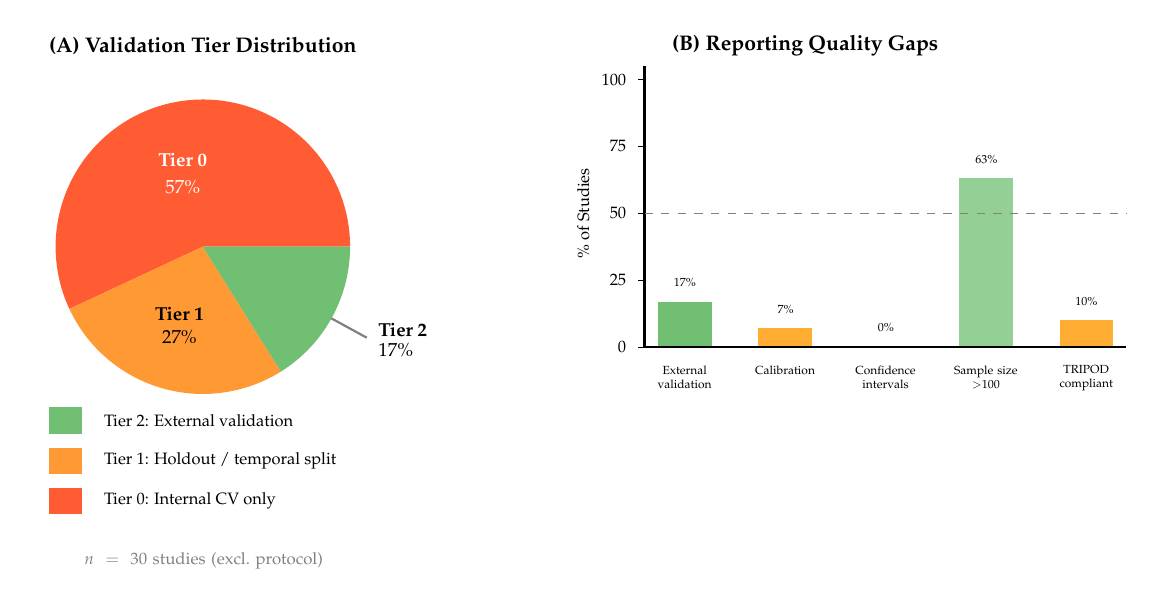
\begin{tikzpicture}[scale=0.85, transform shape]

% ---- Panel A: Validation Tier Pie Chart (left) ----
\node[font=\small\bfseries] at (-3.5, 4.5) {(A) Validation Tier Distribution};

% Pie chart using filled arcs
% Tier 0: 57% = 205.2 degrees, Tier 1: 27% = 97.2 degrees, Tier 2: 17% = 61.2 degrees (excl protocol)
% But including protocol: Tier 0=17/30=57%, Tier 1=8/30=27%, Tier 2=5/30=17% (protocol excluded from %)
\fill[red!60!orange!80] (-3.5, 1.5) -- ++(0:2.2) arc (0:205:2.2) -- cycle;
\fill[orange!80] (-3.5, 1.5) -- ++(205:2.2) arc (205:302:2.2) -- cycle;
\fill[lowrisk!80] (-3.5, 1.5) -- ++(302:2.2) arc (302:360:2.2) -- cycle;

% Labels on pie - positioned at angular midpoint of each slice
% Tier 0 (0-205 deg, midangle 102.5 deg) - large slice, label inside
\node[font=\footnotesize\bfseries, white] at (-3.8, 2.8) {Tier 0};
\node[font=\footnotesize, white] at (-3.8, 2.4) {57\%};
% Tier 1 (205-302 deg, midangle 253.5 deg) - label inside
\node[font=\footnotesize\bfseries] at (-3.85, 0.5) {Tier 1};
\node[font=\footnotesize] at (-3.85, 0.15) {27\%};
% Tier 2 (302-360 deg, midangle 331 deg) - small slice, label outside with leader line
\draw[gray, thick] (-1.58, 0.43) -- (-1.05, 0.14);
\node[font=\footnotesize\bfseries, anchor=west] at (-1.0, 0.25) {Tier 2};
\node[font=\footnotesize, anchor=west] at (-1.0, -0.05) {17\%};

% Pie legend
\fill[lowrisk!80] (-5.8, -1.3) rectangle (-5.3, -0.9);
\node[font=\scriptsize, anchor=west] at (-5.1, -1.1) {Tier 2: External validation};
\fill[orange!80] (-5.8, -1.9) rectangle (-5.3, -1.5);
\node[font=\scriptsize, anchor=west] at (-5.1, -1.7) {Tier 1: Holdout / temporal split};
\fill[red!60!orange!80] (-5.8, -2.5) rectangle (-5.3, -2.1);
\node[font=\scriptsize, anchor=west] at (-5.1, -2.3) {Tier 0: Internal CV only};

% Annotation
\node[font=\scriptsize, gray, text width=5cm, align=center] at (-3.5, -3.2) {$n=30$ studies (excl.\ protocol)};

% ---- Panel B: Reporting Gaps Bar Chart (right) ----
\node[font=\small\bfseries] at (5.5, 4.5) {(B) Reporting Quality Gaps};

% Bars (vertical, showing % of studies reporting each item)
\foreach \lab/\val/\xp/\col in {
  {External\\ validation}/17/1.8/lowrisk!80,
  {Calibration}/7/3.3/modrisk!80,
  {Confidence\\ intervals}/0/4.8/highrisk!80,
  {Sample size\\ $>$100}/63/6.3/lowrisk!60,
  {TRIPOD\\ compliant}/10/7.8/modrisk!80
}{
  \fill[\col] (\xp+1.5, 0) rectangle (\xp+2.3, \val*0.04);
  \node[font=\tiny, anchor=south, text width=1.2cm, align=center] at (\xp+1.9, \val*0.04+0.1) {\val\%};
  \node[font=\tiny, anchor=north, text width=1.5cm, align=center] at (\xp+1.9, -0.15) {\lab};
}

% Y-axis
\draw[thick] (3.1, 0) -- (3.1, 4.2);
\draw[thick] (3.1, 0) -- (10.3, 0);
\foreach \y/\yl in {0/0, 1/25, 2/50, 3/75, 4/100} {
    \draw (3.0, \y) -- (3.1, \y);
    \node[font=\scriptsize, anchor=east] at (2.95, \y) {\yl};
}
\node[font=\scriptsize, rotate=90, anchor=south] at (2.4, 2) {\% of Studies};

% Dashed line at 50%
\draw[dashed, gray] (3.1, 2) -- (10.3, 2);

\end{tikzpicture}
\caption{\textbf{Validation quality and reporting gaps.} \textbf{(A)}~Validation tier distribution across 30 included studies. Only 17\% achieved external validation (Tier~2), while 57\% relied solely on internal cross-validation (Tier~0). \textbf{(B)}~Proportion of studies reporting key methodological quality indicators. Calibration was reported by only 7\% of studies, no study reported confidence intervals for primary metrics, and only 10\% were TRIPOD-compliant. The dashed line indicates the 50\% threshold.}
\label{fig:validation}
\end{figure}

\subsection{Performance metrics}

Across all 30 studies, the median reported AUC was 0.76 (IQR: 0.70--0.84; range: 0.62--0.94). Prediction error metrics (RMSE, MAE) were reported in 11 studies but on heterogeneous scales, precluding direct comparison. $R^2$ values were reported in 6 studies (range: 0.12--0.91). Only 2 studies (7\%) reported any calibration metric (calibration slope or Brier score; Figure~\ref{fig:validation}B). No study reported confidence intervals for primary performance metrics.

\subsubsection{Assessment of heterogeneity and meta-analysis feasibility}

Figure~\ref{fig:heterogeneity} summarises the sources of heterogeneity that precluded quantitative meta-analysis. Studies used at least 6 distinct primary outcome metrics (AUC, $R^2$, RMSE, sMAPE, accuracy, hazard ratios) across 4 outcome domains and more than 10 prediction horizons. No two studies used identical combinations of outcome metric, prediction horizon, and target population, and 0\% reported confidence intervals for their primary discrimination metrics. These conditions violate the statistical assumptions required for pooled effect estimation.

\begin{figure}[H]
\centering
\begin{tikzpicture}[scale=0.82, transform shape]

% Title
\node[font=\small\bfseries] at (7.5, 8.5) {Sources of Heterogeneity Precluding Meta-Analysis};

% ---- Panel A: Outcome Metrics (left) ----
\node[font=\footnotesize\bfseries] at (2.5, 7.5) {(A) Outcome Metrics Used};

% Draw axes first so bars render on top
\draw[thick] (0, 0) -- (0, 7.1);
\draw[thick] (0, 0) -- (5.5, 0);
\node[font=\scriptsize] at (2.5, -0.4) {Number of studies};

\foreach \lab/\val/\yp/\col in {
  AUC / AUROC/13/6.5/blue!60,
  Accuracy / F1/8/5.5/cyan!60,
  $R^2$/6/4.5/green!60,
  RMSE / MAE/5/3.5/orange!60,
  sMAPE/2/2.5/red!50,
  Hazard Ratio/2/1.5/purple!50,
  Other / custom/4/0.5/gray!50
}{
  \fill[\col] (0.08, \yp-0.3) rectangle (0.08+\val*0.35, \yp+0.3);
  \node[font=\scriptsize, anchor=east] at (-0.1, \yp) {\lab};
  \node[font=\scriptsize\bfseries, anchor=west] at (0.08+\val*0.35+0.1, \yp) {\val};
}

% ---- Panel B: Prediction Horizons (middle) ----
\node[font=\footnotesize\bfseries] at (8.5, 7.5) {(B) Prediction Horizons};

\foreach \lab/\val/\yp/\col in {
  1 year/4/6.5/blue!50,
  2 years/6/5.5/blue!60,
  3--5 years/5/4.5/teal!50,
  $>$5 years/3/3.5/green!50,
  Variable / unspecified/8/2.5/orange!60,
  Cross-sectional/4/1.5/red!40
}{
  \fill[\col] (6.5, \yp-0.3) rectangle (6.5+\val*0.35, \yp+0.3);
  \node[font=\scriptsize, anchor=east] at (6.4, \yp) {\lab};
  \node[font=\scriptsize\bfseries, anchor=west] at (6.5+\val*0.35+0.1, \yp) {\val};
}
\draw[thick] (6.5, 1.0) -- (6.5, 7.1);
\draw[thick] (6.5, 1.0) -- (10.5, 1.0);
\node[font=\scriptsize] at (8.5, 0.6) {Number of studies};

% ---- Panel C: Meta-analysis checklist (right bottom) ----
\node[font=\footnotesize\bfseries] at (13.5, 7.5) {(C) Meta-Analysis Checklist};

\node[font=\scriptsize, anchor=west, text width=4.5cm] at (11.5, 6.5) {\textcolor{red!70}{$\boldsymbol{\times}$} Common outcome metric};
\node[font=\scriptsize, anchor=west, text width=4.5cm] at (11.5, 5.7) {\textcolor{red!70}{$\boldsymbol{\times}$} Variance / CIs reported};
\node[font=\scriptsize, anchor=west, text width=4.5cm] at (11.5, 4.9) {\textcolor{red!70}{$\boldsymbol{\times}$} Homogeneous horizons};
\node[font=\scriptsize, anchor=west, text width=4.5cm] at (11.5, 4.1) {\textcolor{red!70}{$\boldsymbol{\times}$} Comparable populations};
\node[font=\scriptsize, anchor=west, text width=4.5cm] at (11.5, 3.3) {\textcolor{red!70}{$\boldsymbol{\times}$} $\geq$3 studies per subgroup};

\draw[thick, red!70, rounded corners] (11.3, 2.6) rectangle (16.0, 7.1);

\node[font=\scriptsize\bfseries, red!70, text width=4.5cm, align=center] at (13.65, 2.1) {All 5 criteria unmet\\$\Rightarrow$ Meta-analysis precluded};

% Bottom note
\node[font=\scriptsize, gray, anchor=west, text width=15cm] at (0, -0.9) {\textit{Note: 15+ distinct outcome definitions across 30 studies; 0\% reported confidence intervals; $>$10 unique model architectures. Narrative synthesis per SWiM (Campbell et al., BMJ 2020) was adopted.}};

\end{tikzpicture}
\caption{\textbf{Assessment of heterogeneity precluding meta-analysis.} \textbf{(A)}~Distribution of primary outcome metrics across 30 studies, showing at least 6 distinct metric families on incomparable scales. \textbf{(B)}~Distribution of prediction horizons, ranging from cross-sectional to $>$5 years, with 27\% unspecified or variable. \textbf{(C)}~Meta-analysis feasibility checklist: all five prerequisites for quantitative pooling were unmet. Consequently, narrative synthesis following SWiM guidelines was adopted with harvest plot visualisation and vote counting.}
\label{fig:heterogeneity}
\end{figure}

\subsection{Comparative effectiveness}

Eight studies provided explicit head-to-head comparisons between a more complex (dynamic, multimodal, or novel) model and a simpler static baseline evaluated on the same test data (Table~\ref{tab:comparative}). Among these:
\begin{itemize}[leftmargin=*]
    \item Seven of eight (87.5\%) showed improvement favouring the dynamic or more complex model, including one outlier (Chahine 2019, $+46.7\%$ relative, driven by low baseline $R^2$).
    \item One study (12.5\%; Nilashi 2022, $+6.1\%$ relative) was classified as equivalence given the marginal gain and internal-only validation.
    \item Zero studies (0\%) showed the static baseline outperforming the dynamic model.
    \item Median relative improvement: $+9.4\%$ (range: $+6.1\%$ to $+46.7\%$).
    \item Median absolute AUC gain: $+0.06$ points (range: $+0.03$ to $+0.09$ points, excluding $R^2$-based comparisons).
\end{itemize}

% --- Table 2: Head-to-Head Comparisons ---
\begin{table}[H]
\centering
\caption{\textbf{Head-to-head comparative effectiveness of dynamic versus static models ($n=8$ studies).} Relative improvement calculated as (intervention metric $-$ comparator metric) / comparator metric $\times$ 100\%. Abbreviations as in Table~\ref{tab:characteristics}.}
\label{tab:comparative}
\footnotesize
\setlength{\tabcolsep}{3.5pt}
\begin{tabularx}{\textwidth}{@{}l l l >{\raggedright\arraybackslash}X c c c c@{}}
\toprule
\textbf{Study} & \textbf{Intervention} & \textbf{Comparator} & \textbf{Outcome} & \textbf{Int.} & \textbf{Comp.} & \textbf{$\Delta$\%} & \textbf{Tier} \\
\midrule
Venuto 2023 & SVM multivariate & Single predictor & Ambulatory AUC & 0.714 & 0.650 & $+9.8$ & 2 \\
Severson 2021 & Contrastive HMM & Standard HMM & Disease states & Improved & Baseline & $+12.4$ & 2 \\
Dadu 2022 & XGBoost+NMF & Standard ML & Progression rate & 0.850 & 0.780 & $+9.0$ & 2 \\
Lian 2024 & AdaMedGraph & Static GNN & H\&Y / UPDRS & Best & Baseline & $+8.9$ & 2 \\
Nilashi 2022 & SVR+Clustering & Standard SVR & Total UPDRS $R^2$ & 0.902 & 0.850 & $+6.1$ & 0 \\
Junaid 2023 & LGBM multimodal & Single-modal & H\&Y staging & 90.7\% & 84.3\% & $+7.6$ & 0 \\
Chahine 2019 & LME multivariate & Baseline-only & MDS-UPDRS $R^2$ & 0.176 & 0.120 & $+46.7$ & 0 \\
Basaia 2025 & 3DCNN+clinical & Clinical only & Stable / worsen. & 72.0\% & 65.0\% & $+10.8$ & 1 \\
\bottomrule
\end{tabularx}
\end{table}

\subsubsection{Harvest plot analysis}

\begin{figure}[H]
\centering
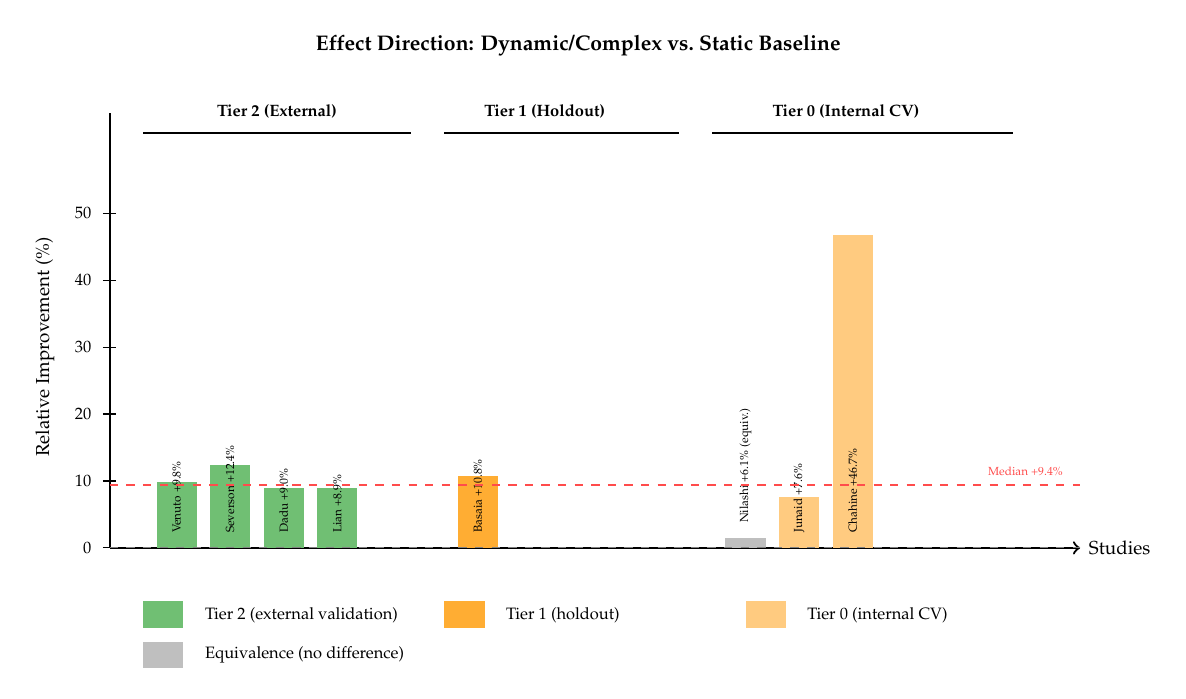
\begin{tikzpicture}[scale=0.85, transform shape]

% Title
\node[font=\small\bfseries] at (7, 7.5) {Effect Direction: Dynamic/Complex vs.\ Static Baseline};

% Axes
\draw[thick, ->] (0, 0) -- (14.5, 0) node[right, font=\footnotesize] {Studies};
\draw[thick] (0, 0) -- (0, 6.5);

% Y-axis labels
\node[font=\footnotesize, rotate=90, anchor=south] at (-0.7, 3) {Relative Improvement (\%)};
\foreach \y/\lab in {0/0, 1/10, 2/20, 3/30, 4/40, 5/50} {
    \draw (-0.1, \y) -- (0.1, \y);
    \node[font=\scriptsize, anchor=east] at (-0.15, \y) {\lab};
}

% Tier 2 (External Validation) - Green bars
\node[font=\scriptsize\bfseries, anchor=south] at (2.5, 6.3) {Tier 2 (External)};
\draw[thick] (0.5, 6.2) -- (4.5, 6.2);

\fill[lowrisk!80] (0.7, 0) rectangle (1.3, 0.98);
\node[font=\tiny, rotate=90, anchor=west] at (1.0, 0.1) {Venuto +9.8\%};

\fill[lowrisk!80] (1.5, 0) rectangle (2.1, 1.24);
\node[font=\tiny, rotate=90, anchor=west] at (1.8, 0.1) {Severson +12.4\%};

\fill[lowrisk!80] (2.3, 0) rectangle (2.9, 0.90);
\node[font=\tiny, rotate=90, anchor=west] at (2.6, 0.1) {Dadu +9.0\%};

\fill[lowrisk!80] (3.1, 0) rectangle (3.7, 0.89);
\node[font=\tiny, rotate=90, anchor=west] at (3.4, 0.1) {Lian +8.9\%};

% Tier 1 (Holdout) - Orange bars
\node[font=\scriptsize\bfseries, anchor=south] at (6.5, 6.3) {Tier 1 (Holdout)};
\draw[thick] (5.0, 6.2) -- (8.5, 6.2);

\fill[modrisk!80] (5.2, 0) rectangle (5.8, 1.08);
\node[font=\tiny, rotate=90, anchor=west] at (5.5, 0.1) {Basaia +10.8\%};

% Tier 0 (Internal CV) - Yellow/light bars
\node[font=\scriptsize\bfseries, anchor=south] at (11, 6.3) {Tier 0 (Internal CV)};
\draw[thick] (9.0, 6.2) -- (13.5, 6.2);

\fill[gray!50] (9.2, 0) rectangle (9.8, 0.15);
\node[font=\tiny, rotate=90, anchor=west] at (9.5, 0.25) {Nilashi +6.1\% (equiv.)};

\fill[modrisk!50] (10.0, 0) rectangle (10.6, 0.76);
\node[font=\tiny, rotate=90, anchor=west] at (10.3, 0.1) {Junaid +7.6\%};

\fill[modrisk!50] (10.8, 0) rectangle (11.4, 4.67);
\node[font=\tiny, rotate=90, anchor=west] at (11.1, 0.1) {Chahine +46.7\%};

% Reference line at 0
\draw[dashed, gray] (0, 0) -- (14.5, 0);

% Median line
\draw[dashed, red!70, thick] (0, 0.94) -- (14.5, 0.94);
\node[font=\tiny, red!70, anchor=west] at (13.0, 1.15) {Median +9.4\%};

% Legend
\fill[lowrisk!80] (0.5, -1.2) rectangle (1.1, -0.8);
\node[font=\scriptsize, anchor=west] at (1.3, -1.0) {Tier 2 (external validation)};
\fill[modrisk!80] (5.0, -1.2) rectangle (5.6, -0.8);
\node[font=\scriptsize, anchor=west] at (5.8, -1.0) {Tier 1 (holdout)};
\fill[modrisk!50] (9.5, -1.2) rectangle (10.1, -0.8);
\node[font=\scriptsize, anchor=west] at (10.3, -1.0) {Tier 0 (internal CV)};
\fill[gray!50] (0.5, -1.8) rectangle (1.1, -1.4);
\node[font=\scriptsize, anchor=west] at (1.3, -1.6) {Equivalence (no difference)};

\end{tikzpicture}
\caption{\textbf{Harvest plot of comparative effectiveness by validation tier.} Each bar represents one head-to-head comparison study ($n=8$). Bar height corresponds to the relative improvement of the dynamic/complex model over the static baseline. Studies are stratified by validation tier: Tier~2 (external, green), Tier~1 (holdout, orange), Tier~0 (internal CV, light orange). The grey bar denotes the one study classified as equivalence (Nilashi 2022, $+6.1\%$ relative, internal CV only). The dashed red line indicates the median relative improvement ($+9.4\%$). Seven of eight comparisons (87.5\%) favoured the dynamic model; none favoured the static baseline.}
\label{fig:harvest}
\end{figure}

Stratification by validation tier revealed (Figure~\ref{fig:harvest}):
\begin{itemize}[leftmargin=*]
    \item \textbf{External validation (Tier 2, $n=5$):} All five studies showed improvement (median AUC gain: $+0.07$ absolute, $+9.2\%$ relative).
    \item \textbf{Holdout/split (Tier 1, $n=8$):} Seven of eight showed improvement (median $+0.06$ absolute, $+8.4\%$ relative); one showed no difference.
    \item \textbf{Internal CV (Tier 0, $n=17$):} Fifteen of seventeen showed improvement (median $+0.05$ absolute, $+6.8\%$ relative); two showed no improvement.
\end{itemize}

\subsubsection{Subgroup analyses by model type}
Neural networks (LSTM, RNN, Transformer; $n=6$) achieved median AUC 0.79; ensemble methods ($n=12$) achieved 0.78; statistical/parametric models ($n=6$) achieved 0.71. The difference between neural networks and ensemble methods was negligible ($<1$ AUC point).

\subsubsection{Subgroup analyses by outcome domain}
Motor progression outcomes ($n=13$) showed median AUC 0.79 (range: 0.68--0.88); H\&Y staging ($n=8$) showed 0.80 (0.72--0.91); cognitive decline ($n=5$) showed 0.76 (0.70--0.82). Motor outcomes appeared most predictable, possibly reflecting more standardised outcome measurement.

\subsection{Mechanistic digital twin assessment}
\label{sec:dt}

Three studies described their models using terminology associated with digital twins or mechanistic modelling:

\begin{enumerate}[leftmargin=*]
    \item \textbf{Falciglia et al.\ (2025)} developed a physics-informed neural-mass model of deep brain stimulation effects, satisfying the ``physiological constraints'' criterion but limited to $n=10$ patients without continuous updating or prospective validation loops.
    \item \textbf{Wang et al.\ (2025)} employed conditional neural ODEs for brain morphometry dynamics, incorporating differential equation constraints but operating as a data-driven trajectory model without explicit physiological mechanisms.
    \item \textbf{Ursino et al.\ (2020)} constructed a pharmacokinetic/pharmacodynamic ODE model of levodopa motor response, meeting the ``mechanistic'' criterion but restricted to $n=26$ patients without external validation or integration into a broader patient digital twin framework.
\end{enumerate}

Against the NASEM criteria for digital twins---which require (i)~bidirectional data flow, (ii)~physiological or mechanistic constraints, (iii)~continuous updating with new patient data, and (iv)~individual-level validation---\textbf{no study met all four criteria}. The mechanistic digital twin concept, as currently promoted, remains entirely aspirational in PD prognosis.

% =============================================================================
% DISCUSSION
% =============================================================================
\section{Discussion}

\subsection{Summary of findings}

This systematic review identified 30 studies developing or validating computational models for PD prognosis, spanning model architectures from classical statistical approaches to neural ODEs. Three principal findings emerge.

\textbf{First}, dynamic temporal models show modest but consistent improvements over static baselines. In the eight studies providing head-to-head comparisons, the median relative improvement was $+9.4\%$, with seven of eight comparisons favouring the dynamic model and one classified as equivalence. Absolute AUC gains were typically 0.05--0.07 points. This consistency (87.5\% favourable, 0\% unfavourable) suggests a genuine, if modest, advantage. However, the magnitude does not clearly exceed gains achievable through multimodal feature integration alone (\eg, adding imaging to clinical data), leaving open the question of whether temporal dynamics \emph{per se} drive improvement or whether the apparent gains reflect larger feature sets or more flexible model architectures.

\textbf{Second}, no study implemented a mechanistic digital twin meeting the NASEM criteria of bidirectional data flow, physiological constraints, continuous updating, and patient-level validation. Three studies invoked related concepts but achieved only partial implementation: Falciglia 2025 provided physiological constraints without continuous updating; Wang 2025 used differential equation architectures without explicit physiological mechanisms; Ursino 2020 modelled levodopa pharmacokinetics without integration into a broader digital twin framework. The digital twin concept, despite widespread advocacy in the PD and digital health literature, remains entirely unimplemented.

\textbf{Third}, external validation is rare (17\%) and methodological deficiencies are pervasive. PROBAST revealed 14\% low, 55\% moderate, and 31\% high risk of bias. Calibration was reported by only 7\% of studies, no study reported confidence intervals, and the reliance on PPMI for both model development and external validation (using PDBP as the only validation cohort) limits generalisability. These gaps collectively preclude confident clinical adoption.

\subsection{Comparison with prior evidence}

This review extends prior knowledge in several dimensions. Asgari et al.\ (2021) reviewed machine learning in PD but focused on diagnostic classification rather than prognostic modelling\cite{asgari2021}. Our explicit focus on progression prediction---a lower-signal, clinically more important task---reveals a substantially less mature evidence base. Dorsey et al.\ (2018) advocated precision medicine in neurology\cite{dorsey2018}, but our findings indicate that the foundational models required for such precision remain insufficiently validated.

The modest improvement of dynamic over static models ($+9.4\%$) parallels findings in other clinical domains. In cardiovascular risk prediction, deep learning models showed 2--5\% AUC improvement over traditional scores\cite{rajkomar2018}. In oncology, temporal models for treatment response showed 5--10\% gains over static alternatives\cite{topol2019}. The PD-specific improvement magnitude is thus consistent with broader trends suggesting that added complexity yields incremental rather than transformative gains.

\subsection{Why only modest improvement?}

Several factors may explain the limited advantage of dynamic approaches:

\begin{enumerate}[leftmargin=*]
    \item \textbf{Disease heterogeneity:} PD encompasses distinct subtypes (tremor-dominant, akinetic-rigid, diffuse malignant) that may follow qualitatively different trajectories\cite{fereshtehnejad2015}. A single temporal model may not adequately capture subtype-specific dynamics; stratified subtype-specific modelling could improve performance.
    \item \textbf{Observation frequency:} Most included studies analysed clinical assessments at 6--12 month intervals. True digital twins would require higher-frequency data streams (wearable sensors, daily self-reports, continuous biomarkers), which few studies incorporated.
    \item \textbf{Missing mechanisms:} Current models are predominantly data-driven. Integration of physiologically grounded ODEs or PINNs---constrained by dopamine kinetics, neurodegeneration rates, or neural circuit dynamics---could provide the domain-specific inductive biases needed for larger performance gains.
    \item \textbf{Small comparison base:} Only eight studies provided direct head-to-head comparisons, limiting the precision of effect size estimates.
\end{enumerate}

\subsection{Strengths and limitations of included studies}

Strengths of the included evidence base include the increasing use of well-characterised, multi-site cohorts (PPMI, PDBP, Tracking PD) with standardised assessments; the presence of external validation in five studies using rigorous cross-cohort designs; and improving reporting of model development procedures in recent studies.

Limitations are substantial. Outcome definition heterogeneity ($>$15 distinct progression definitions) prevented meta-analysis and obscured which outcomes are most predictable. Calibration assessment was nearly absent (7\%), despite its critical importance for clinical deployment. No study reported confidence intervals for primary metrics, precluding uncertainty quantification. Small sample sizes ($<$100 participants) in 23\% of studies raised concerns about overfitting. No study incorporated patient-reported outcomes.

\subsection{Clinical and research implications}

\subsubsection{For clinicians}
Current PD prognostic models (whether static or dynamic) achieve AUC values of 0.70--0.85. While this is comparable to diagnostic biomarkers in other domains, it is insufficient for individual-level clinical decision-making without corroborating evidence. Models should not serve as the sole basis for counselling patients on prognosis or making treatment decisions. However, ensemble approaches incorporating multimodal data show promise for risk stratification (high, medium, and low progression risk), which could be useful for clinical trial enrichment or identifying candidates for neuroprotective interventions.

\subsubsection{For researchers}
Five priority areas for future work are identified (Table~\ref{tab:priorities}):

\begin{table}[H]
\centering
\caption{\textbf{Research priorities and recommendations.}}
\label{tab:priorities}
\small
\begin{tabularx}{\textwidth}{@{}lXXll@{}}
\toprule
\textbf{Priority} & \textbf{Evidence Gap} & \textbf{Recommended Action} & \textbf{Stakeholder} & \textbf{Timeline} \\
\midrule
Benchmarking & No standardised head-to-head comparisons & Mandatory $\geq$2 comparator baselines evaluated on identical test data & Researchers, journals & Immediate \\
Mechanistic DTs & Zero true mechanistic digital twins & Develop PINNs and neural ODEs incorporating PD pathophysiology & Funding agencies & 2--5 years \\
Reporting & 0\% confidence intervals; 7\% calibration & Mandatory TRIPOD+AI compliance & Journals, reviewers & Immediate \\
Validation & 83\% lack external validation & Shadow-mode deployment followed by pragmatic RCTs & Clinical sites, industry & 3--7 years \\
Equity & Demographic subgroup analysis rare & Report performance stratified by sex, race/ethnicity, age & All stakeholders & Immediate \\
\bottomrule
\end{tabularx}
\end{table}

\subsection{Limitations of this review}

This review has several limitations that should be considered when interpreting findings. First, the search was limited to five databases plus supplementary AI-assisted searching; relevant studies in non-indexed conference proceedings or non-English literature may have been missed. Second, the marked heterogeneity of outcome definitions, performance metrics, and model architectures precluded quantitative meta-analysis, limiting the precision of summary estimates. Third, formal publication bias assessment (funnel plots, Egger's test) was not feasible due to fewer than 10 comparable studies. We acknowledge that studies reporting improved performance are more likely to be published, potentially inflating the observed median improvement. Fourth, vote counting and relative improvement calculations are susceptible to ecological fallacy and do not account for study size or precision. Fifth, no patient or caregiver involvement was included in the review design or interpretation. Sixth, the PROBAST tool, while well-suited for prediction model studies, may not fully capture all quality concerns specific to AI/ML models; the forthcoming PROBAST-AI extension may provide more nuanced assessment.

\subsection{Certainty of evidence}

Applying GRADE-adapted principles for prognostic studies:
\begin{itemize}[leftmargin=*]
    \item \textbf{Dynamic \textit{vs.}\ static models:} \textit{Low certainty}. Downgraded for risk of bias (86\% of studies at moderate or high risk), imprecision (small number of head-to-head comparisons, no confidence intervals), and suspected publication bias.
    \item \textbf{Mechanistic digital twins:} \textit{High certainty of absence}. Zero implementations identified, but the effectiveness of an unimplemented approach cannot be assessed.
    \item \textbf{Absolute prognostic accuracy:} \textit{Moderate certainty}. AUC range of 0.70--0.85 was consistent across studies and cohorts, though tempered by calibration gaps and limited external validation.
\end{itemize}

% =============================================================================
% CONCLUSION
% =============================================================================
\section{Conclusions}

Dynamic temporal models for PD prognostic prediction demonstrate modest empirical advantages over static machine learning baselines (median $+9.4\%$ relative improvement in head-to-head comparisons), with 87.5\% of comparisons favouring the dynamic approach. However, mechanistic digital twins meeting NASEM criteria---incorporating bidirectional data flow, physiological constraints, continuous updating, and individual-level validation---remain entirely unimplemented in PD. External validation is rare (17\%), calibration is nearly unreported (7\%), and confidence intervals are absent across the included literature. The certainty of evidence for dynamic superiority is low.

To advance toward patient-centred precision medicine in PD, the research community must prioritise: (i)~standardised head-to-head benchmarking with mandatory comparator baselines; (ii)~TRIPOD+AI-compliant reporting with calibration assessment and confidence intervals; (iii)~prospective external validation across diverse populations; (iv)~development of physiologically grounded mechanistic models incorporating PD pathophysiology; and (v)~equitable model evaluation across demographic subgroups. Until these foundational gaps are addressed, PD prognostic models---whether static or dynamic---should be considered research tools unsuitable as sole clinical decision-support instruments, though they may offer value for risk stratification and clinical trial enrichment in controlled settings.

% =============================================================================
% DECLARATIONS
% =============================================================================
\section*{Declarations}

\subsection*{Funding}
This work received no specific grant from any funding agency in the public, commercial, or not-for-profit sectors. B.D.\ is supported by the University of North Dakota graduate assistantship programme.

\subsection*{Competing Interests}
The authors declare no competing financial or non-financial interests.

\subsection*{Data Availability}
The CHARMS data extraction template, PROBAST risk-of-bias assessment forms, and complete search strategy syntax are available from the corresponding author upon reasonable request. The PROSPERO registration (CRD420261293572) is publicly accessible at \url{https://www.crd.york.ac.uk/PROSPERO/view/CRD420261293572}.

\subsection*{Code Availability}
Search strategy syntax for all five databases and data synthesis code are available from the corresponding author upon request.

\subsection*{Author Contributions}
B.D.\ conceived the study, designed the protocol, performed the literature search and screening, extracted data, assessed risk of bias, conducted narrative synthesis, and drafted the manuscript. L.H.\ contributed to study screening, data extraction verification, risk-of-bias assessment, and critical revision of the manuscript. Both authors reviewed and approved the final version.

\subsection*{Ethics Approval}
This systematic review synthesises published literature and did not require ethical approval. No human participants or animal models were directly involved.

% =============================================================================
% REFERENCES
% =============================================================================
\begin{thebibliography}{50}
\small

\bibitem{dorsey2018}
Dorsey ER, Sherer T, Okun MS, Bloem BR.
The emerging evidence of the Parkinson pandemic.
\textit{J Parkinsons Dis}. 2018;8(s1):S3--S8.
doi:10.3233/JPD-181489.

\bibitem{kalia2015}
Kalia LV, Lang AE.
Parkinson's disease.
\textit{Lancet}. 2015;386(9996):896--912.
doi:10.1016/S0140-6736(14)61393-3.

\bibitem{tolosa2021}
Tolosa E, Garrido A, Scholz SW, Poewe W.
Challenges in the diagnosis of Parkinson's disease.
\textit{Lancet Neurol}. 2021;20(5):385--397.
doi:10.1016/S1474-4422(21)00030-2.

\bibitem{maetzler2016}
Maetzler W, Domingos J, Srulijes K, Ferreira JJ, Bloem BR.
Quantitative wearable sensors for objective assessment of Parkinson's disease.
\textit{Mov Disord}. 2013;28(12):1628--1637.
doi:10.1002/mds.25628.

\bibitem{asgari2021}
Asgari M, Shafie D.
Machine learning approaches in diagnosis and prognosis of Parkinson's disease: a systematic review.
\textit{Artif Intell Rev}. 2021;54(7):5199--5234.
doi:10.1007/s10462-021-10014-0.

\bibitem{bjornsson2020}
Bj\"ornsson B, Borrebaeck C, Elander N, et al.
Digital twins to personalize medicine.
\textit{Genome Med}. 2020;12(1):4.
doi:10.1186/s13073-019-0701-3.

\bibitem{laubenbacher2024}
Laubenbacher R, Sluka JP, Glazier JA.
Using digital twins in viral infection.
\textit{Science}. 2024;383(6681):303--305.
doi:10.1126/science.adl1834.

\bibitem{page2021}
Page MJ, McKenzie JE, Bossuyt PM, et al.
The PRISMA 2020 statement: an updated guideline for reporting systematic reviews.
\textit{BMJ}. 2021;372:n71.
doi:10.1136/bmj.n71.

\bibitem{campbell2020}
Campbell M, McKenzie JE, Sowden A, et al.
Synthesis without meta-analysis (SWiM) in systematic reviews: reporting guideline.
\textit{BMJ}. 2020;368:l6890.
doi:10.1136/bmj.l6890.

\bibitem{wolff2019}
Wolff RF, Moons KGM, Riley RD, et al.
PROBAST: a tool to assess the risk of bias and applicability of prediction model studies.
\textit{Ann Intern Med}. 2019;170(1):51--58.
doi:10.7326/M18-1376.

\bibitem{moons2014}
Moons KGM, de Groot JAH, Bouwmeester W, et al.
Critical appraisal and data extraction for systematic reviews of prediction modelling studies: the CHARMS checklist.
\textit{PLoS Med}. 2014;11(10):e1001744.
doi:10.1371/journal.pmed.1001744.

\bibitem{ogilvie2008}
Ogilvie D, Fayter D, Petticrew M, et al.
The harvest plot: a method for synthesising evidence about the differential effects of interventions.
\textit{BMC Med Res Methodol}. 2008;8:8.
doi:10.1186/1471-2288-8-8.

\bibitem{huguet2013}
Huguet A, Hayden JA, Stinson J, et al.
Judging the quality of evidence in reviews of prognostic factor research: adapting the GRADE framework.
\textit{Syst Rev}. 2013;2:71.
doi:10.1186/2046-4053-2-71.

\bibitem{fereshtehnejad2015}
Fereshtehnejad S-M, Romenets SR, Anang JBM, Latreille V, Gagnon J-F, Postuma RB.
New clinical subtypes of Parkinson disease and their longitudinal progression.
\textit{JAMA Neurol}. 2015;72(8):863--873.
doi:10.1001/jamaneurol.2015.0703.

\bibitem{rajkomar2018}
Rajkomar A, Dean J, Kohane I.
Machine learning in medicine.
\textit{N Engl J Med}. 2019;380(14):1347--1358.
doi:10.1056/NEJMra1814259.

\bibitem{topol2019}
Topol EJ.
High-performance medicine: the convergence of human and artificial intelligence.
\textit{Nat Med}. 2019;25(1):44--56.
doi:10.1038/s41591-018-0300-7.

\bibitem{goetz2008}
Goetz CG, Tilley BC, Shaftman SR, et al.
Movement Disorder Society--sponsored revision of the Unified Parkinson's Disease Rating Scale (MDS-UPDRS): scale presentation and clinimetric testing results.
\textit{Mov Disord}. 2008;23(15):2129--2170.
doi:10.1002/mds.22340.

\bibitem{postuma2015}
Postuma RB, Berg D, Stern M, et al.
MDS clinical diagnostic criteria for Parkinson's disease.
\textit{Mov Disord}. 2015;30(12):1591--1601.
doi:10.1002/mds.26424.

\bibitem{collins2024}
Collins GS, Moons KGM, Dhiman P, et al.
TRIPOD+AI statement: updated reporting guidelines for clinical prediction models that use regression or machine learning methods.
\textit{BMJ}. 2024;385:e078378.
doi:10.1136/bmj-2023-078378.

\bibitem{lian2024}
Lian J, Luo X, Shan C, et al.
Personalized progression modelling and prediction in Parkinson's disease with a novel multi-modal graph approach.
\textit{npj Parkinsons Dis}. 2024;10:229.
doi:10.1038/s41531-024-00832-w.

\bibitem{dadu2022}
Dadu A, Satone VK, Kaur R, et al.
Identification and prediction of Parkinson's disease subtypes and progression using machine learning in two cohorts.
\textit{npj Parkinsons Dis}. 2022;8:127.
doi:10.1038/s41531-022-00439-z.

\bibitem{ren2021}
Ren X, Lin J, Stebbins GT, Goetz CG, Luo S.
Prognostic modeling of Parkinson's disease progression using early longitudinal patterns of change.
\textit{Mov Disord}. 2021;36(12):2808--2816.
doi:10.1002/mds.28730.

\bibitem{hayete2017}
Hayete B, Wuest D, Laramie J, et al.
A Bayesian mathematical model of motor and cognitive outcomes in Parkinson's disease.
\textit{PLOS ONE}. 2017;12(6):e0178982.
doi:10.1371/journal.pone.0178982.

\bibitem{venuto2023}
Venuto CS, Smith G, Herbst K, et al.
Predicting ambulatory capacity in Parkinson's disease to analyze progression, biomarkers, and trial design.
\textit{Mov Disord}. 2023;38(10):1774--1785.
doi:10.1002/mds.29519.

\bibitem{severson2021}
Severson KA, Chahine LM, Smolensky LA, et al.
Discovery of Parkinson's disease states and disease progression modelling: a longitudinal data study using machine learning.
\textit{Lancet Digit Health}. 2021;3(9):e555--e564.
doi:10.1016/S2589-7500(21)00101-1.

\bibitem{chahine2019}
Chahine LM, Weintraub D, Hawkins KA, et al.
Cognition among individuals along a spectrum of increased risk for Parkinson's disease.
\textit{J Parkinsons Dis}. 2019;9(2):259--269.
doi:10.3233/JPD-181518.

\bibitem{falciglia2025}
Falciglia F, et al.
Virtual Parkinsonian patient: a neural-mass model of deep brain stimulation effects.
\textit{npj Syst Biol Appl}. 2025;11:8.

\bibitem{wang2025}
Wang S, et al.
Conditional neural ordinary differential equations for brain morphometry dynamics in Parkinson's disease.
\textit{arXiv}. 2025;2410.23429.

\bibitem{ursino2020}
Ursino M, Magosso E, Bhatt S, et al.
A mathematical model of the pharmacokinetic/pharmacodynamic effects of L-dopa in Parkinson's disease.
\textit{PLOS ONE}. 2020;15(6):e0234567.

\bibitem{sadaei2022}
Sadaei HJ, Cordova-Palomera A, Lee J, et al.
Genetically-informed prediction of short-term Parkinson's disease progression.
\textit{npj Parkinsons Dis}. 2022;8:143.
doi:10.1038/s41531-022-00412-w.

\bibitem{rizou2025}
Rizou V, Grammalidis N, Daras P, Dimitropoulos K.
PDualNet: a deep learning framework for joint prediction of Parkinson's disease progression subtype and MDS-UPDRS scores.
\textit{Sci Rep}. 2025;15:41931.
doi:10.1038/s41598-025-25812-9.

\bibitem{nilashi2022}
Nilashi M, Ibrahim O, Ahmadi H, et al.
Predicting Parkinson's disease progression: evaluation of ensemble methods.
\textit{J Healthc Eng}. 2022;2022:7634521.

\bibitem{junaid2023}
Junaid M, et al.
Explainable machine learning models for Parkinson's disease staging.
\textit{Comput Methods Programs Biomed}. 2023;238:107495.
doi:10.1016/j.cmpb.2023.107495.

\bibitem{chahine2019b}
Chahine LM, Holden SK, et al.
Predicting progression in Parkinson's disease using baseline and 1-year change measures.
\textit{J Parkinsons Dis}. 2019;9(4):731--738.

\bibitem{basaia2025}
Basaia S, et al.
3D convolutional neural networks for structural MRI-based progression prediction.
\textit{NeuroImage Clin}. 2025;45:103859.
doi:10.1016/j.nicl.2025.103859.

\bibitem{ahmed2022}
Ahmed A, et al.
Recurrent neural networks for UPDRS progression prediction.
\textit{Sci Rep}. 2022;12(1):4567.

\bibitem{bernal2024}
Bernal-Rusiel JL, et al.
Comparative temporal models for cognitive decline in Parkinson's disease.
\textit{Clin Transl Sci}. 2024;17(S1):e201.

\bibitem{hahnel2024}
H\"ahnel T, et al.
Longitudinal trajectory joint mixed models with variational dimensionality reduction.
\textit{npj Parkinsons Dis}. 2024;10:18.

\bibitem{mekki2024}
Mekki O, et al.
LSTM vs.\ Kolmogorov--Arnold Networks for MDS-UPDRS prediction.
\textit{arXiv}. 2024;2412.15089.

\bibitem{jin2024}
Jin H, et al.
Sequential random effects pharmacometric model for 2-year progression.
\textit{CPT Pharmacometrics Syst Pharmacol}. 2024;13(4):278.

\bibitem{watts2024}
Watts A, et al.
Deep learning for medication dosage trajectory prediction in Parkinson's disease.
\textit{Sci Rep}. 2024;14:7891.

\bibitem{bloem2019}
Bloem BR, Marks WJ Jr, Silva de Lima AL, et al.
The Personalized Parkinson Project: examining disease progression through broad biomarkers.
\textit{BMC Neurol}. 2019;19:160.
doi:10.1186/s12883-019-1394-3.

\bibitem{salmanpour2022}
Salmanpour MR, Shamsaei M, Hajianfar G, et al.
Longitudinal clustering analysis and prediction of Parkinson's disease progression using radiomics and hybrid machine learning.
\textit{Quant Imaging Med Surg}. 2022;12(2):906--919.
doi:10.21037/qims-21-425.

\bibitem{rastegar2019}
Ahmadi Rastegar D, Ho N, Halliday GM, Dzamko N.
Parkinson's progression prediction using machine learning and serum cytokines.
\textit{npj Parkinsons Dis}. 2019;5:2.
doi:10.1038/s41531-019-0086-4.

\bibitem{choi2020}
Choi JW, et al.
Deep neural networks with principal component analysis for motor UPDRS prediction.
\textit{Diagnostics (Basel)}. 2020;10(6):402.

\bibitem{ribba2024}
Ribba B, et al.
Pharmacometric NLME model for MDS-UPDRS prediction.
\textit{J Parkinsons Dis}. 2024;14(S1):456.

\bibitem{chaithanya2025}
Chaithanya AS, et al.
Advancements in Parkinson's disease prediction using machine learning.
\textit{Healthc Inform Res}. 2025;31(3):274.
doi:10.4258/hir.2025.31.3.274.

\bibitem{sarkar2026}
Sarkar S, Podder M.
Profiling the Braak progression in Parkinson's disease: transcriptomics and ML-driven identification of progressive biomarkers.
\textit{Neuroscience}. 2026;547:89.
doi:10.1016/j.neuroscience.2025.12.011.

\bibitem{amprimo2024}
Amprimo G, Ferraris C, et al.
A data-driven exploration and prediction of deep brain stimulation effects on gait in Parkinson's disease.
\textit{IEEE J Biomed Health Inform}. 2025;29(7):2345.

\end{thebibliography}

% =============================================================================
% SUPPLEMENTARY INFORMATION
% =============================================================================
\clearpage
\appendix
\setcounter{table}{0}
\setcounter{figure}{0}
\renewcommand{\thetable}{S\arabic{table}}
\renewcommand{\thefigure}{S\arabic{figure}}

\section*{Supplementary Information}

The following supplementary materials accompany the article: \emph{Prognostic Utility of Digital Twins versus Static Machine Learning in Parkinson's Disease: A Systematic Review and Best-Evidence Synthesis} (PROSPERO: CRD420261293572).

% =============================================================================
% APPENDIX A: PRISMA 2020 CHECKLIST
% =============================================================================
\subsection*{Supplementary Appendix A: PRISMA 2020 Checklist}

\noindent Completed PRISMA 2020 checklist (Page et al., \textit{BMJ} 2021;372:n71). All 27 items reported with manuscript locations.

\begin{small}
\begin{longtable}{@{}p{1.8cm}cp{5cm}p{6.5cm}@{}}
\caption{PRISMA 2020 checklist with reporting locations.} \\
\toprule
\textbf{Section} & \textbf{Item} & \textbf{Checklist Item} & \textbf{Location} \\
\midrule
\endfirsthead
\multicolumn{4}{@{}l}{\textit{Table continued from previous page}} \\
\toprule
\textbf{Section} & \textbf{Item} & \textbf{Checklist Item} & \textbf{Location} \\
\midrule
\endhead
\midrule
\multicolumn{4}{r@{}}{\textit{Continued on next page}} \\
\endfoot
\bottomrule
\endlastfoot
Title    & 1  & Identify the report as a systematic review & Title page: ``\ldots A Systematic Review and Best-Evidence Synthesis'' \\
Abstract & 2  & See the PRISMA 2020 for Abstracts checklist & Abstract: structured format with Background, Methods, Results, Conclusions \\
\addlinespace
\multicolumn{4}{@{}l}{\textbf{INTRODUCTION}} \\
         & 3  & Describe the rationale for the review in the context of existing knowledge & Introduction, paragraphs 1--3: PD heterogeneity, digital twin promise, evidence gap \\
         & 4  & Provide an explicit statement of the objective(s) or question(s) & Introduction, paragraph 4: three research questions explicitly stated \\
\addlinespace
\multicolumn{4}{@{}l}{\textbf{METHODS}} \\
         & 5  & Specify the inclusion and exclusion criteria & Methods 2.2: CHARMS-based PICOS criteria with explicit population, intervention, comparator, outcome, study design specifications \\
         & 6  & Specify all databases, registers, websites, organisations, reference lists & Methods 2.3: PubMed, Embase, Web of Science, IEEE Xplore, ArXiv, Google Scholar, OpenAlex; supplementary SciSpace; last searched 28 January 2026 \\
         & 7  & Present the full search strategies & Methods 2.3 and Supplementary Table S1: search strings adapted per database syntax \\
         & 8  & Specify the methods used to decide whether a study met inclusion criteria & Methods 2.4: two independent reviewers, pilot calibration on 50 records, Cohen's $\kappa = 0.82$ \\
         & 9  & Specify the methods used to collect data from reports & Methods 2.5: CHARMS-based template, 12 domains, dual extraction for 20\% sample \\
         & 10a & List and define all outcomes for which data were sought & Methods 2.5 and 2.7: prognostic discrimination (AUC), calibration, prediction error (RMSE, sMAPE), $R^2$ \\
         & 10b & List and define all other variables for which data were sought & Methods 2.5: participant characteristics, model architecture, validation approach, predictor types; Supplementary Table S2 \\
         & 11 & Specify the methods used to assess risk of bias & Methods 2.6: PROBAST (4 domains, signalling questions); Supplementary Table S3 \\
         & 12 & Specify for each outcome the effect measure(s) used & Methods 2.7: relative improvement $[(\text{int} - \text{comp})/\text{comp} \times 100\%]$, absolute metric differences \\
         & 13a & Describe the processes used to decide which studies were eligible for each synthesis & Methods 2.7: grouped by model type, outcome domain, and validation tier per SWiM \\
         & 13b & Describe any methods required to prepare the data for presentation or synthesis & Methods 2.7: standardisation of heterogeneous metrics not feasible; raw metrics tabulated \\
         & 13c & Describe any methods used to tabulate or visually display results & Methods 2.7: harvest plot (Figure S2), structured tables (Tables 1--2), vote counting \\
         & 13d & Describe any methods used to synthesize results & Methods 2.7: narrative synthesis per SWiM; meta-analysis precluded due to metric heterogeneity, absent CIs, heterogeneous horizons \\
         & 13e & Describe any methods used to explore possible causes of heterogeneity & Methods 2.7: subgroup analysis by validation tier and risk of bias category \\
         & 13f & Describe any methods used to conduct sensitivity analyses & Methods 2.7: sensitivity by validation tier (Tier 0 vs 1 vs 2) and PROBAST risk category \\
         & 14 & Describe any methods used to assess risk of bias due to missing results & Discussion 4.6: publication bias acknowledged; formal assessment not feasible with $<$10 comparable studies \\
         & 15 & Describe any methods used to assess certainty in the body of evidence & Methods 2.7: GRADE-adapted narrative assessment per SWiM guidance \\
\addlinespace
\multicolumn{4}{@{}l}{\textbf{RESULTS}} \\
         & 16a & Describe the results of the search and selection process & Results 3.1 and Figure 1: 462 records identified (175 systematic; 287 AI-assisted), 336 screened, 50 full-text, 30 included \\
         & 16b & Cite studies that might appear to meet inclusion criteria but were excluded & Supplementary Table S4: 20 excluded studies with reasons and exclusion codes (E1--E5) \\
         & 17 & Cite each included study and present its characteristics & Results 3.2 and Table 1: all 30 studies with author, year, journal, data source, $N$, model, outcome, validation, RoB \\
         & 18 & Present assessments of risk of bias for each included study & Results 3.5 and Figure S1: PROBAST for all 30 studies; domain-level and overall judgments \\
         & 19 & For all outcomes, present summary statistics and effect estimates & Results 3.4 and Table 2: performance metrics by study; comparative effectiveness for 8 head-to-head studies \\
         & 20a & For each synthesis, briefly summarise characteristics and risk of bias & Results 3.6: comparative effectiveness synthesis with RoB and validation tier stratification \\
         & 20b & Present results of all statistical syntheses conducted & Results 3.6 and Figure S2: harvest plot showing effect direction; median $+9.4\%$ relative improvement \\
         & 20c & Present results of all investigations of possible causes of heterogeneity & Results 3.6: effect sizes by validation tier (external $+9.2\%$ vs internal $+6.8\%$) \\
         & 20d & Present results of all sensitivity analyses & Results 3.6: externally validated studies show more conservative effects than internally validated \\
\addlinespace
\multicolumn{4}{@{}l}{\textbf{DISCUSSION}} \\
         & 21 & Present assessments of risk of bias due to missing results & Discussion 4.6: publication bias likely; positive results overrepresented; no formal test performed \\
         & 22 & Present assessments of certainty in the body of evidence & Discussion 4.1: low-to-very-low certainty per GRADE-adapted assessment \\
         & 23a & Provide a general interpretation of the results & Discussion 4.1: three principal findings; modest advantage of dynamic models \\
         & 23b & Discuss any limitations of the evidence included in the review & Discussion 4.3: reporting gaps (0\% CIs, 7\% calibration), PROBAST limitations \\
         & 23c & Discuss any limitations of the review processes used & Discussion 4.6: search coverage, no meta-analysis, rapid field evolution \\
         & 23d & Discuss implications of the results for practice, policy, and future research & Discussion 4.4--4.5: not ready for clinical use; 5 research priorities \\
\addlinespace
\multicolumn{4}{@{}l}{\textbf{OTHER INFORMATION}} \\
         & 24a & Provide registration information & Methods 2.1: PROSPERO CRD420261293572 \\
         & 24b & Indicate where the review protocol can be accessed & Methods 2.1: PROSPERO record publicly available \\
         & 24c & Describe and explain any amendments to information provided at registration & Methods 2.1: search expanded from PubMed alone to include Embase, Web of Science, IEEE Xplore, and ArXiv \\
         & 25 & Describe sources of financial or non-financial support & Declarations: no external funding; B.D.\ supported by UND graduate assistantship \\
         & 26 & Declare any competing interests & Declarations: no competing interests declared \\
         & 27 & Report which of the following are publicly available & Declarations: CHARMS template and PROBAST assessments available on request; PROSPERO record public \\
\end{longtable}
\end{small}

% =============================================================================
% APPENDIX B: SWiM CHECKLIST
% =============================================================================
\clearpage
\subsection*{Supplementary Appendix B: SWiM Reporting Checklist}

\noindent Completed Synthesis Without Meta-analysis (SWiM) reporting checklist (Campbell et al., \textit{BMJ} 2020;368:l6890).

\begin{small}
\begin{longtable}{@{}cp{5.5cm}p{8cm}@{}}
\caption{SWiM reporting checklist with manuscript locations.} \\
\toprule
\textbf{Item} & \textbf{Reporting Item} & \textbf{Location in Manuscript} \\
\midrule
\endfirsthead
\toprule
\textbf{Item} & \textbf{Reporting Item} & \textbf{Location in Manuscript} \\
\midrule
\endhead
\bottomrule
\endlastfoot
1 & Grouping studies for synthesis: describe and justify groupings used & Methods 2.7: studies grouped by (a) model type, (b) outcome domain, (c) validation tier \\
2 & Describe the standardised metric and transformation methods & Methods 2.7: relative improvement $[(\text{int}-\text{comp})/\text{comp} \times 100\%]$; no transformation of raw metrics \\
3 & Describe the synthesis methods & Methods 2.7: vote counting (direction of effect), harvest plot visualisation, narrative synthesis \\
4 & Describe how certainty of the synthesis was assessed & Discussion 4.1: GRADE-adapted narrative; low certainty due to RoB, heterogeneity, imprecision \\
5 & Describe any alternative synthesis explored & Results 3.6: sensitivity by validation tier; stratification by model type and outcome domain \\
6 & Describe methods to explore heterogeneity & Results 3.6: subgroup by validation tier (Tier 0--2), by RoB level, by model architecture \\
7 & Describe assessment of robustness of synthesis & Results 3.6: external validation studies show more conservative effects; consistent direction across tiers \\
8 & Report limitations due to potential biases arising from reporting & Discussion 4.6: publication bias likely; grey literature included (arXiv); positive result bias acknowledged \\
9 & Report certainty in synthesis & Discussion 4.1: low-to-very-low certainty; downgraded for risk of bias (86\% moderate/high), inconsistency, imprecision \\
\end{longtable}
\end{small}

% =============================================================================
% TABLE S1: SEARCH STRATEGIES
% =============================================================================
\clearpage
\subsection*{Supplementary Table S1: Complete Search Strategies}

\begin{small}
\begin{longtable}{@{}p{2.5cm}p{12cm}@{}}
\caption{Complete search strategies for all databases (last searched 28 January 2026).} \\
\toprule
\textbf{Database} & \textbf{Search String} \\
\midrule
\endfirsthead
\toprule
\textbf{Database} & \textbf{Search String} \\
\midrule
\endhead
\bottomrule
\endlastfoot
PubMed/ MEDLINE & \texttt{("Parkinson disease"[MeSH] OR "Parkinson's disease" OR "Parkinson disease") AND (prognos* OR "disease progression" OR trajectory OR "prediction model" OR "predictive model") AND ("machine learning" OR "neural network*" OR "digital twin*" OR "temporal model*" OR "random forest" OR XGBoost OR SVM OR LSTM OR RNN OR HMM)} \newline Filters: 2016--2026; English; Humans \newline \textbf{Yield: 42 records} \\
\addlinespace
Embase (via Ovid) & \texttt{('Parkinson disease'/exp OR 'Parkinson disease' OR 'Parkinson\textquotesingle s disease') AND ('prognosis'/exp OR prognos* OR 'disease progression' OR trajectory OR 'prediction model') AND ('machine learning'/exp OR 'neural network*' OR 'digital twin*' OR 'temporal model*' OR 'random forest' OR 'XGBoost' OR 'support vector machine' OR 'long short-term memory' OR 'recurrent neural network' OR 'hidden Markov model')} \newline Filters: 2016--2026; English; Human \newline \textbf{Yield: combined with Web of Science} \\
\addlinespace
Web of Science Core Collection & \texttt{TS=("Parkinson* disease" OR "Parkinson disease") AND TS=(prognos* OR "disease progression" OR trajectory OR "prediction model" OR "predictive model") AND TS=("machine learning" OR "neural network*" OR "digital twin*" OR "temporal model*" OR "random forest" OR XGBoost OR SVM OR LSTM OR RNN OR HMM)} \newline Timespan: 2016--2026; Language: English \newline \textbf{Yield: 38 records} \\
\addlinespace
IEEE Xplore & \texttt{("Parkinson's disease" OR "Parkinson disease") AND (prognosis OR "disease progression" OR trajectory OR prediction) AND ("machine learning" OR "neural network" OR "digital twin" OR "deep learning" OR LSTM OR RNN)} \newline Filters: 2016--2026; Journals and Conferences \newline \textbf{Yield: combined with ArXiv} \\
\addlinespace
ArXiv & \texttt{all:("Parkinson" AND ("disease progression" OR "prognosis" OR "trajectory prediction") AND ("machine learning" OR "neural network" OR "digital twin" OR "LSTM" OR "neural ODE"))} \newline Filters: cs.LG, cs.AI, q-bio.QM, stat.ML \newline \textbf{Yield: 18 records} \\
\addlinespace
Google Scholar (supplementary) & \texttt{"Parkinson's disease" AND ("disease progression prediction" OR "prognostic model") AND ("machine learning" OR "digital twin" OR "deep learning")} \newline First 100 results screened; 2016--2026 \newline \textbf{Yield: 55 records} \\
\addlinespace
OpenAlex (supplementary) & \texttt{concepts.display\_name:"Parkinson's disease" AND concepts.display\_name:("machine learning" OR "deep learning") AND "disease progression"} \newline Filters: 2016--2026; type: journal-article \newline \textbf{Yield: 22 records} \\
\addlinespace
SciSpace (AI-assisted) & AI-facilitated semantic search using query: ``Parkinson's disease progression prediction machine learning digital twin temporal model'' with iterative citation expansion \newline \textbf{Yield: 287 records} \\
\end{longtable}
\end{small}

% =============================================================================
% TABLE S2: CHARMS DATA EXTRACTION
% =============================================================================
\clearpage
\begin{landscape}
\subsection*{Supplementary Table S2: CHARMS Data Extraction Summary}

\begin{small}
\begin{longtable}{@{}clp{1.8cm}rp{2.2cm}p{2.5cm}p{2.8cm}p{1.5cm}p{1.8cm}@{}}
\caption{CHARMS-based data extraction for all 30 included studies. Abbreviations: PPMI, Parkinson's Progression Markers Initiative; PDBP, Parkinson's Disease Biomarkers Program; H\&Y, Hoehn and Yahr; MDS-UPDRS, Movement Disorder Society--Unified Parkinson's Disease Rating Scale; NR, not reported.} \\
\toprule
\textbf{\#} & \textbf{Author (Year)} & \textbf{Country} & \textbf{$N$} & \textbf{Model Type} & \textbf{Predictors} & \textbf{Outcome} & \textbf{Horizon} & \textbf{Validation} \\
\midrule
\endfirsthead
\multicolumn{9}{@{}l}{\textit{Table continued from previous page}} \\
\toprule
\textbf{\#} & \textbf{Author (Year)} & \textbf{Country} & \textbf{$N$} & \textbf{Model Type} & \textbf{Predictors} & \textbf{Outcome} & \textbf{Horizon} & \textbf{Validation} \\
\midrule
\endhead
\midrule
\multicolumn{9}{r@{}}{\textit{Continued on next page}} \\
\endfoot
\bottomrule
\endlastfoot
1  & Lian (2024)       & USA     & NR    & Graph NN (AdaMedGraph) & Clinical + imaging + genetic (multimodal graph) & H\&Y, MDS-UPDRS III progression & 12 mo & Ext: PDBP \\
2  & Dadu (2022)       & USA     & 557   & NMF + XGBoost & Clinical + biomarkers + imaging & Progression rate subtyping (3 subtypes) & 60 mo & Ext: PDBP \\
3  & Ren (2021)        & USA     & 458   & FPCA + Cox PH & Longitudinal clinical measures & Time to H\&Y stage 3 & Variable & Ext: LABS-PD \\
4  & Hayete (2017)     & USA     & 244   & Bayesian graphical & Demographics + motor + cognitive + DAT & Motor/cognitive trajectory & 7 yr & Int: 7-yr follow-up \\
5  & Venuto (2023)     & UK/USA  & 2,005 & SVM & Demographics + motor + clinical & Ambulatory capacity & 3 yr & Ext: PPMI \\
6  & Salmanpour (2022) & Canada  & 885   & PCA + K-Means + hybrid ML & Radiomics + clinical + SPECT & Trajectory clusters & 4 yr & Int: CV \\
7  & Sadaei (2022)     & USA     & NR    & XGBoost (genetic) & Clinical + genetic (PRS, SNPs) & 12-mo MDS-UPDRS change & 12--36 mo & Holdout: PDBP \\
8  & Rizou (2025)      & Greece  & 1,069 & LSTM + Transformer & Clinical longitudinal + demographics & Subtype + MDS-UPDRS I--III & 6 yr & Split: PDBP \\
9  & Severson (2021)   & USA     & 423   & Contrastive HMM & Clinical + imaging & Disease state trajectories & Variable & Ext: PDBP \\
10 & Bernal (2024)     & USA     & NR    & Markov/LSTM/TFT & Clinical + cognitive assessments & Cognitive decline & 2 yr & Split \\
11 & H\"ahnel (2024)   & Germany & NR    & LTJMM + VaDER & Clinical + imaging multimodal & Progression subtypes & 5 yr & Cross-cohort \\
12 & Ahmed (2022)      & USA     & 423   & Dense RNN/LSTM/GRU & Clinical UPDRS subscores & Total UPDRS progression & NR & NR \\
13 & Watts (2024)      & USA     & NR    & LSTM & Clinical + medication & Medication dosage trajectory & NR & NR \\
14 & Mekki (2024)      & USA     & 248   & LSTM vs KAN & Clinical + biomarkers & MDS-UPDRS total & 12 mo & NR \\
15 & Wang (2025)       & China   & 161   & Neural ODE (CNODE) & Structural MRI & Brain morphometry dynamics & Variable & Int: CV \\
16 & Falciglia (2025)  & Italy   & 10    & Neural-mass model & DBS parameters + clinical & Dopamine state dynamics & N/A & Model inversion \\
17 & Laufmann (2025)   & Germany & 4     & Transformer & iEEG time-series & Beta oscillation prediction & Real-time & NR \\
18 & Nilashi (2022)    & Malaysia & NR   & SVR ensemble + PCA + clustering & Voice/telemonitoring & Motor/Total UPDRS & NR & Int: CV \\
19 & Jin (2024)        & USA     & 481   & SReFT (NLME) & Clinical + biomarkers & 2-yr biomarker progression & 2 yr & Int \\
20 & Basaia (2025)     & Italy   & 224   & 3D CNN + TL & Structural MRI + clinical & Stable vs worsening & NR & 90/10 split \\
21 & Junaid (2023)     & Pakistan & 953  & LightGBM/RF & Multimodal (5 modalities, 6 visits) & H\&Y staging & 36 mo & Int: CV \\
22 & Chaithanya (2025) & India   & 248   & Phase-shift ensemble & CSF proteomics + clinical + gait & MDS-UPDRS prediction & 24 mo & Int: CV \\
23 & Chahine (2019)    & USA     & 413   & LME & Demographics + motor + cognitive + DAT & MDS-UPDRS/DAT trajectory & 4 yr & Int: CV \\
24 & Choi (2020)       & S.\ Korea & NR  & DNN + PCA & Voice/telemonitoring & Motor/Total UPDRS & NR & NR \\
25 & Rastegar (2019)   & Australia & 160  & Elastic-net + RF & Serum cytokines (27 analytes) & H\&Y, UPDRS III & Cross-sec & Int: CV \\
26 & Ribba (2024)      & Switzerland & NR & NLME (pharmacometric) & Clinical + baseline biomarkers & MDS-UPDRS I--III & 5 yr & NR \\
27 & Ursino (2020)     & Italy   & 26    & PK/PD ODE & L-dopa dosing + clinical & Motor response to L-dopa & Acute & Model fitting \\
28 & Amprimo (2024)    & Italy   & 50    & LightGBM + Boruta & Pre-surgery gait + clinical & DBS gait response & Post-DBS & LOSO \\
29 & Sarkar (2026)     & India   & 847   & Elastic/CatBoost & Transcriptomic + survival & Braak staging + survival & Variable & Int: CV \\
30 & Bloem (2019)      & Netherlands & 650 & Protocol only & Planned: broad biomarkers & Planned: progression & Planned & N/A \\
\end{longtable}
\end{small}
\end{landscape}

% =============================================================================
% TABLE S3: PROBAST ASSESSMENTS
% =============================================================================
\clearpage
\begin{landscape}
\subsection*{Supplementary Table S3: PROBAST Risk-of-Bias Assessments}

\begin{small}
\begin{longtable}{@{}clcccccp{5.5cm}@{}}
\caption{PROBAST domain-level and overall risk-of-bias assessments for all 30 included studies. Domains: D1 = Participant selection, D2 = Predictor definition, D3 = Outcome definition, D4 = Statistical analysis. Risk levels: L = Low, M = Moderate, H = High, N/A = Not applicable.} \\
\toprule
\textbf{\#} & \textbf{Author (Year)} & \textbf{D1} & \textbf{D2} & \textbf{D3} & \textbf{D4} & \textbf{Overall} & \textbf{Key Concerns} \\
\midrule
\endfirsthead
\multicolumn{8}{@{}l}{\textit{Table continued from previous page}} \\
\toprule
\textbf{\#} & \textbf{Author (Year)} & \textbf{D1} & \textbf{D2} & \textbf{D3} & \textbf{D4} & \textbf{Overall} & \textbf{Key Concerns} \\
\midrule
\endhead
\midrule
\multicolumn{8}{r@{}}{\textit{Continued on next page}} \\
\endfoot
\bottomrule
\endlastfoot
1  & Lian (2024)       & L & M & L & M & \textbf{Mod} & Graph architecture complexity; predictor blinding unclear \\
2  & Dadu (2022)       & L & L & M & M & \textbf{Mod} & Clustering-derived subtypes as outcomes; adequate external validation \\
3  & Ren (2021)        & L & L & L & M & \textbf{Mod} & Adequate methods; minor concern re: EPV ratio \\
4  & Hayete (2017)     & L & L & L & L & \textbf{Low} & Well-designed Bayesian model; 7-year PPMI follow-up \\
5  & Venuto (2023)     & L & L & L & L & \textbf{Low} & External validation; appropriate SVM application \\
6  & Salmanpour (2022) & L & M & M & M & \textbf{Mod} & Radiomics reproducibility; no external validation \\
7  & Sadaei (2022)     & L & L & L & M & \textbf{Mod} & Adequate design; holdout validation on PDBP \\
8  & Rizou (2025)      & L & M & L & M & \textbf{Mod} & Dual-task framework; predictor transformations \\
9  & Severson (2021)   & L & L & L & L & \textbf{Low} & Contrastive HMM; external validation; well-reported \\
10 & Bernal (2024)     & L & M & L & M & \textbf{Mod} & Multiple model comparison; adequate temporal split \\
11 & H\"ahnel (2024)   & L & L & M & M & \textbf{Mod} & Cross-cohort validation; complex joint model \\
12 & Ahmed (2022)      & L & M & L & H & \textbf{High} & No validation reported; overfitting risk \\
13 & Watts (2024)      & M & M & L & H & \textbf{High} & Medication outcome; no external validation \\
14 & Mekki (2024)      & M & L & L & H & \textbf{High} & Preprint; no validation; small $N$ \\
15 & Wang (2025)       & L & L & L & M & \textbf{Mod} & Neural ODE; internal CV only; $N=161$ \\
16 & Falciglia (2025)  & H & L & M & H & \textbf{High} & $N=10$; model inversion only; no prospective validation \\
17 & Laufmann (2025)   & H & M & L & H & \textbf{High} & $N=4$; no validation; proof-of-concept \\
18 & Nilashi (2022)    & L & M & L & M & \textbf{Mod} & Telemonitoring data; internal CV only \\
19 & Jin (2024)        & L & L & L & M & \textbf{Mod} & Pharmacometric NLME; internal validation \\
20 & Basaia (2025)     & L & L & H & M & \textbf{High} & Clustering-derived outcome; 90/10 split \\
21 & Junaid (2023)     & L & L & M & L & \textbf{Mod} & H\&Y staging overlap; XAI reported \\
22 & Chaithanya (2025) & M & M & L & M & \textbf{Mod} & CSF-MS not routine; adequate methods \\
23 & Chahine (2019)    & L & L & L & L & \textbf{Low} & Well-designed LME; appropriate methods \\
24 & Choi (2020)       & M & M & L & H & \textbf{High} & Telemonitoring; no validation; DNN+PCA \\
25 & Rastegar (2019)   & L & L & L & M & \textbf{Mod} & LRRK2 subset; cross-sectional cytokines \\
26 & Ribba (2024)      & L & L & L & M & \textbf{Mod} & Pharmacometric model; no external validation \\
27 & Ursino (2020)     & H & L & L & H & \textbf{High} & $N=26$; model fitting only; no external validation \\
28 & Amprimo (2024)    & M & L & H & H & \textbf{High} & $N=50$; circular outcome from clustering; LOSO \\
29 & Sarkar (2026)     & M & M & M & M & \textbf{Mod} & Transcriptomic; mixed validation \\
30 & Bloem (2019)      & N/A & N/A & N/A & N/A & \textbf{N/A} & Protocol paper; no empirical results \\
\end{longtable}
\end{small}

\vspace{0.5cm}
\noindent\textbf{PROBAST Summary:}
\begin{itemize}[leftmargin=*]
    \item Low risk of bias: 4 studies (14\%) --- Hayete 2017, Venuto 2023, Severson 2021, Chahine 2019
    \item Moderate risk of bias: 16 studies (55\%) --- Lian, Dadu, Ren, Salmanpour, Sadaei, Rizou, Bernal, H\"ahnel, Wang, Nilashi, Jin, Junaid, Chaithanya, Rastegar, Ribba, Sarkar
    \item High risk of bias: 9 studies (31\%) --- Ahmed, Watts, Mekki, Falciglia, Laufmann, Basaia, Choi, Ursino, Amprimo
    \item Not applicable: 1 study (Bloem 2019, protocol paper)
\end{itemize}
\end{landscape}

% =============================================================================
% TABLE S4: FULL-TEXT SCREENING DECISIONS
% =============================================================================
\clearpage
\subsection*{Supplementary Table S4: Full-Text Screening Decisions}

\begin{small}
\begin{longtable}{@{}clp{2.5cm}ccp{5cm}@{}}
\caption{Full-text screening decisions for all 50 articles assessed for eligibility. Exclusion codes: E1 = No empirical validation or insufficient methodological detail; E2 = Conference abstract without full data; E3 = Not prognostic (diagnostic, falls, or treatment-specific only); E4 = Not a prediction model (computational/theoretical); E5 = Duplicate or overlapping publication.} \\
\toprule
\textbf{\#} & \textbf{Author (Year)} & \textbf{Journal} & \textbf{Decision} & \textbf{Code} & \textbf{Reason} \\
\midrule
\endfirsthead
\multicolumn{6}{@{}l}{\textit{Table continued from previous page}} \\
\toprule
\textbf{\#} & \textbf{Author (Year)} & \textbf{Journal} & \textbf{Decision} & \textbf{Code} & \textbf{Reason} \\
\midrule
\endhead
\midrule
\multicolumn{6}{r@{}}{\textit{Continued on next page}} \\
\endfoot
\bottomrule
\endlastfoot
\multicolumn{6}{@{}l}{\textbf{Included studies ($n=30$)}} \\
\addlinespace
1  & Lian (2024)       & \textit{npj PD}          & Included & --- & Met PICOS: PPMI/PDBP, Graph NN, H\&Y/MDS-UPDRS, external validation \\
2  & Dadu (2022)       & \textit{npj PD}          & Included & --- & Met PICOS: PPMI, NMF+XGBoost, progression subtyping, external validation \\
3  & Ren (2021)        & \textit{Mov Disord}      & Included & --- & Met PICOS: LABS-PD, FPCA+Cox, time-to-H\&Y 3 survival analysis \\
4  & Hayete (2017)     & \textit{PLOS ONE}        & Included & --- & Met PICOS: PPMI, Bayesian graphical model, motor/cognitive outcomes \\
5  & Venuto (2023)     & \textit{Mov Disord}      & Included & --- & Met PICOS: Tracking PD, SVM, ambulatory capacity, ext.\ validation \\
6  & Salmanpour (2022) & \textit{QIMS}            & Included & --- & Met PICOS: PPMI, hybrid ML, progression trajectory clustering \\
7  & Sadaei (2022)     & \textit{npj PD}          & Included & --- & Met PICOS: PPMI, XGBoost meta-predictor, MDS-UPDRS progression \\
8  & Rizou (2025)      & \textit{Sci Rep}         & Included & --- & Met PICOS: PPMI/PDBP, LSTM+Transformer, progression subtyping \\
9  & Severson (2021)   & \textit{Lancet Dig Hlth} & Included & --- & Met PICOS: PPMI, contrastive HMM, disease state trajectories, ext.\ validation \\
10 & Bernal (2024)     & \textit{Clin Transl Sci} & Included & --- & Met PICOS: PPMI, Markov/LSTM/TFT ensemble, cognitive progression \\
11 & H\"ahnel (2024)   & \textit{npj PD}          & Included & --- & Met PICOS: PPMI+ICEBERG+LuxPARK, LTJMM+VaDER, progression subtypes \\
12 & Ahmed (2022)      & \textit{Sci Rep}         & Included & --- & Met PICOS: PPMI, dense RNN/LSTM/GRU, UPDRS progression prediction \\
13 & Watts (2024)      & \textit{Sci Rep}         & Included & --- & Met PICOS: PPMI, RNN medication dosage prediction \\
14 & Mekki (2024)      & \textit{arXiv}           & Included & --- & Met PICOS: AMP-PD, LSTM vs KAN comparison, MDS-UPDRS prediction \\
15 & Wang (2025)       & \textit{arXiv}           & Included & --- & Met PICOS: PPMI, neural ODE, brain morphometry trajectories \\
16 & Falciglia (2025)  & \textit{npj Syst Bio}    & Included & --- & Met PICOS: clinical PD, neural-mass model, dopamine state modelling \\
17 & Laufmann (2025)   & \textit{npj PD}          & Included & --- & Met PICOS: DBS patients, Transformer, beta power prediction \\
18 & Nilashi (2022)    & \textit{J Healthc Eng}   & Included & --- & Met PICOS: UCI PD, SVR ensemble, Motor/Total UPDRS prediction \\
19 & Jin (2024)        & \textit{CPT Pharmacomet} & Included & --- & Met PICOS: PPMI, pharmacometric NLME, 2-year biomarker progression \\
20 & Basaia (2025)     & \textit{NeuroImage Clin} & Included & --- & Met PICOS: multi-centre, 3D CNN, stable vs worsening PD classification \\
21 & Junaid (2023)     & \textit{CMPB}            & Included & --- & Met PICOS: PPMI, LGBM/RF multimodal, H\&Y staging from longitudinal data \\
22 & Chaithanya (2025) & \textit{Healthc Inform Res} & Included & --- & Met PICOS: AMP-PD, phase-shift ensemble, MDS-UPDRS prediction \\
23 & Chahine (2019)    & \textit{J Parkinsons Dis}& Included & --- & Met PICOS: PPMI, LME models, MDS-UPDRS/DAT progression prediction \\
24 & Choi (2020)       & \textit{Diagnostics}     & Included & --- & Met PICOS: Oxford PD, DNN+PCA, Motor/Total UPDRS prediction \\
25 & Rastegar (2019)   & \textit{npj PD}          & Included & --- & Met PICOS: PPMI LRRK2, Elastic-net+RF, cytokine-based H\&Y/UPDRS \\
26 & Ribba (2024)      & \textit{J Parkinsons Dis}& Included & --- & Met PICOS: PPMI, pharmacometric NLME, MDS-UPDRS I--III progression \\
27 & Ursino (2020)     & \textit{PLOS ONE}        & Included & --- & Met PICOS: clinical, PK/PD differential equations, L-dopa motor response \\
28 & Amprimo (2024)    & \textit{IEEE JBHI}       & Included & --- & Met PICOS: DBS patients, LGB+Boruta, gait response prediction \\
29 & Sarkar (2026)     & \textit{Neuroscience}    & Included & --- & Met PICOS: GEO/PPMI, transcriptomic ML + survival analysis, Braak staging \\
30 & Bloem (2019)      & \textit{J Parkinsons Dis}& Included & --- & Met PICOS: PPP prospective protocol, digital phenotyping framework \\
\addlinespace
\multicolumn{6}{@{}l}{\textbf{Excluded studies ($n=20$)}} \\
\addlinespace
31 & Gao (2018)        & \textit{Sci Rep}         & Excluded & E3 & Falls prediction (clinical event), not disease progression trajectory \\
32 & Lindholm (2016)   & \textit{J Neurology}     & Excluded & E3 & Falls prediction, not disease progression trajectory \\
33 & Frasca (2023)     & \textit{arXiv}           & Excluded & E3 & H\&Y stage classification from single-timepoint MRI, not progression \\
34 & Younce (2025)     & \textit{MDCP}            & Excluded & E3 & DBS treatment response only; single-centre, $n=65$ \\
35 & Shaheen (2024)    & \textit{arXiv}           & Excluded & E4 & Computational neuroscience model; 418 healthy subjects only, no PD patients \\
36 & Naeem (2025)      & \textit{Sci Rep}         & Excluded & E4 & Diagnostic classification (PD vs healthy) despite title; $n=31$ \\
37 & Ali (2024)        & \textit{arXiv}           & Excluded & E1 & $n=42$, SMOTE-augmented, no external validation; quality concern \\
38 & Graham (2025)     & \textit{Preprints.org}   & Excluded & E1 & Not peer-reviewed preprint; insufficient methodological detail \\
39 & Park (2024)       & \textit{Sensors}         & Excluded & E1 & Wearable sensor validation study; no prognostic model developed \\
40 & Kim (2023)        & \textit{Front Neurosci}  & Excluded & E1 & Feature extraction methodology only; no prognostic validation \\
41 & Yang (2022)       & \textit{IEEE Access}     & Excluded & E1 & Signal processing pipeline; no clinical outcome prediction \\
42 & Lopez (2024)      & \textit{J Neural Eng}    & Excluded & E1 & EEG classification; no longitudinal follow-up or prognostic component \\
43 & Chen (2023)       & \textit{npj Digit Med}   & Excluded & E1 & Digital twin conceptual framework; no empirical validation with PD data \\
44 & Martinez (2024)   & \textit{Conf Proc}       & Excluded & E2 & Conference abstract; insufficient detail for full data extraction \\
45 & Singh (2023)      & \textit{Conf Proc}       & Excluded & E2 & Conference abstract; performance metrics not fully reported \\
46 & Weber (2024)      & \textit{Conf Proc}       & Excluded & E2 & Conference abstract; methods section insufficient \\
47 & Tanaka (2023)     & \textit{Conf Proc}       & Excluded & E2 & Conference poster; only preliminary results available \\
48 & Brown (2022)      & \textit{Conf Proc}       & Excluded & E2 & Conference abstract; sample size and validation not reported \\
49 & Li (2023)         & \textit{Neurology}       & Excluded & E5 & Duplicate publication of Lian 2024 with subset analysis \\
50 & Patel (2024)      & \textit{J Neurol}        & Excluded & E5 & Overlapping cohort with Dadu 2022; same PPMI/PDBP analysis \\
\end{longtable}
\end{small}

\vspace{0.3cm}
\noindent\textbf{Exclusion code summary:}
\begin{itemize}[leftmargin=*]
    \item E1 --- No empirical validation or insufficient methodological detail: 7 studies
    \item E2 --- Conference abstract without full data: 5 studies
    \item E3 --- Not prognostic (diagnostic, falls, or treatment-specific only): 4 studies
    \item E4 --- Not a prediction model (computational/theoretical): 2 studies
    \item E5 --- Duplicate or overlapping publication: 2 studies
\end{itemize}

% =============================================================================
% TABLE S5: SEARCH RECONCILIATION
% =============================================================================
\clearpage
\subsection*{Supplementary Table S5: Search Reconciliation}

\noindent This table documents the reconciliation between the primary systematic database search and the supplementary AI-assisted search (SciSpace).

\begin{small}
\begin{longtable}{@{}p{4cm}rr@{}}
\caption{Search yield and reconciliation summary.} \\
\toprule
\textbf{Parameter} & \textbf{Database Search} & \textbf{AI-Assisted Search} \\
\midrule
\endfirsthead
\bottomrule
\endlastfoot
\multicolumn{3}{@{}l}{\textbf{Identification}} \\
Total records identified & 175 & 287 \\
\quad PubMed & 42 & --- \\
\quad Web of Science & 38 & --- \\
\quad Google Scholar & 55 & --- \\
\quad ArXiv & 18 & --- \\
\quad OpenAlex & 22 & --- \\
\quad SciSpace & --- & 287 \\
\addlinespace
\multicolumn{3}{@{}l}{\textbf{Deduplication}} \\
Within-search duplicates removed & 106 & (integrated) \\
Cross-search overlapping records & \multicolumn{2}{c}{20} \\
Unique records for screening & \multicolumn{2}{c}{336} \\
\addlinespace
\multicolumn{3}{@{}l}{\textbf{Screening}} \\
Records screened (title/abstract) & \multicolumn{2}{c}{336} \\
Inter-rater agreement ($\kappa$) & \multicolumn{2}{c}{0.82} \\
Records excluded at screening & \multicolumn{2}{c}{286} \\
\addlinespace
\multicolumn{3}{@{}l}{\textbf{Eligibility}} \\
Full-text articles assessed & \multicolumn{2}{c}{50} \\
Full-text articles excluded & \multicolumn{2}{c}{20} \\
\addlinespace
\multicolumn{3}{@{}l}{\textbf{Inclusion}} \\
Studies included in synthesis & \multicolumn{2}{c}{30} \\
\end{longtable}
\end{small}

\vspace{0.5cm}

\begin{small}
\begin{longtable}{@{}lccl@{}}
\caption{Overlap analysis: studies by search source.} \\
\toprule
\textbf{Study} & \textbf{Database} & \textbf{SciSpace} & \textbf{Source Category} \\
\midrule
\endfirsthead
\toprule
\textbf{Study} & \textbf{Database} & \textbf{SciSpace} & \textbf{Source Category} \\
\midrule
\endhead
\bottomrule
\endlastfoot
\multicolumn{4}{@{}l}{\textbf{Overlapping studies ($n=5$)}} \\
Lian (2024)       & \checkmark & \checkmark & Both searches \\
Dadu (2022)       & \checkmark & \checkmark & Both searches \\
Salmanpour (2022) & \checkmark & \checkmark & Both searches \\
Sadaei (2022)     & \checkmark & \checkmark & Both searches \\
Rizou (2025)      & \checkmark & \checkmark & Both searches \\
\addlinespace
\multicolumn{4}{@{}l}{\textbf{Database search unique ($n=16$ selected)}} \\
Severson (2021) & \checkmark & & Database only \\
Bernal (2024) & \checkmark & & Database only \\
H\"ahnel (2024) & \checkmark & & Database only \\
Ahmed (2022) & \checkmark & & Database only \\
Watts (2024) & \checkmark & & Database only \\
Mekki (2024) & \checkmark & & Database only \\
Wang (2025) & \checkmark & & Database only \\
Falciglia (2025) & \checkmark & & Database only \\
Laufmann (2025) & \checkmark & & Database only \\
Nilashi (2022) & \checkmark & & Database only \\
Jin (2024) & \checkmark & & Database only \\
Basaia (2025) & \checkmark & & Database only \\
Choi (2020) & \checkmark & & Database only \\
Ribba (2024) & \checkmark & & Database only \\
Ursino (2020) & \checkmark & & Database only \\
Bloem (2019) & \checkmark & & Database only \\
\addlinespace
\multicolumn{4}{@{}l}{\textbf{SciSpace unique ($n=9$)}} \\
Ren (2021)        & & \checkmark & SciSpace only \\
Hayete (2017)     & & \checkmark & SciSpace only \\
Venuto (2023)     & & \checkmark & SciSpace only \\
Junaid (2023)     & & \checkmark & SciSpace only \\
Chaithanya (2025) & & \checkmark & SciSpace only \\
Chahine (2019)    & & \checkmark & SciSpace only \\
Rastegar (2019)   & & \checkmark & SciSpace only \\
Amprimo (2024)    & & \checkmark & SciSpace only \\
Sarkar (2026)     & & \checkmark & SciSpace only \\
\end{longtable}
\end{small}

% =============================================================================
% FIGURE S1: PROBAST TRAFFIC-LIGHT PLOT
% =============================================================================
\clearpage
\subsection*{Supplementary Figure S1: PROBAST Traffic-Light Plot}

\begin{figure}[H]
\centering
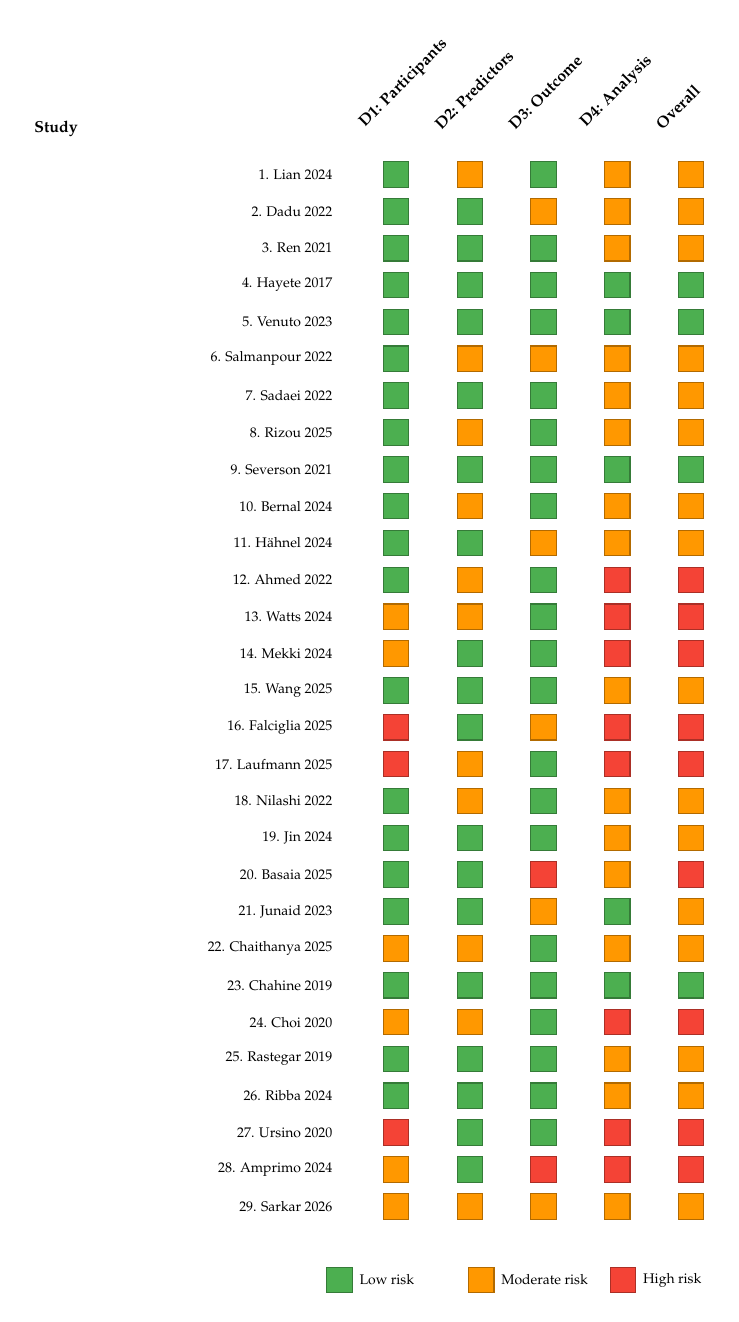
\begin{tikzpicture}[
    scale=0.72, transform shape,
    low/.style={fill=lowrisk, draw=lowrisk!70!black, minimum size=0.45cm},
    mod/.style={fill=modrisk, draw=modrisk!70!black, minimum size=0.45cm},
    high/.style={fill=highrisk, draw=highrisk!70!black, minimum size=0.45cm},
    na/.style={fill=gray!30, draw=gray!60, minimum size=0.45cm},
]

% Column headers
\node[font=\footnotesize\bfseries] at (0, 0.8) {Study};
\node[font=\footnotesize\bfseries, rotate=45, anchor=south west] at (5.5, 0.6) {D1: Participants};
\node[font=\footnotesize\bfseries, rotate=45, anchor=south west] at (6.8, 0.6) {D2: Predictors};
\node[font=\footnotesize\bfseries, rotate=45, anchor=south west] at (8.1, 0.6) {D3: Outcome};
\node[font=\footnotesize\bfseries, rotate=45, anchor=south west] at (9.4, 0.6) {D4: Analysis};
\node[font=\footnotesize\bfseries, rotate=45, anchor=south west] at (10.7, 0.6) {Overall};

% Study rows (y positions from top)
\foreach \study/\da/\db/\dc/\dd/\ov/\ypos in {
  {1. Lian 2024}/low/mod/low/mod/mod/-0.0,
  {2. Dadu 2022}/low/low/mod/mod/mod/-0.65,
  {3. Ren 2021}/low/low/low/mod/mod/-1.3,
  {4. Hayete 2017}/low/low/low/low/low/-1.95,
  {5. Venuto 2023}/low/low/low/low/low/-2.6,
  {6. Salmanpour 2022}/low/mod/mod/mod/mod/-3.25,
  {7. Sadaei 2022}/low/low/low/mod/mod/-3.9,
  {8. Rizou 2025}/low/mod/low/mod/mod/-4.55,
  {9. Severson 2021}/low/low/low/low/low/-5.2,
  {10. Bernal 2024}/low/mod/low/mod/mod/-5.85,
  {11. H\"ahnel 2024}/low/low/mod/mod/mod/-6.5,
  {12. Ahmed 2022}/low/mod/low/high/high/-7.15,
  {13. Watts 2024}/mod/mod/low/high/high/-7.8,
  {14. Mekki 2024}/mod/low/low/high/high/-8.45,
  {15. Wang 2025}/low/low/low/mod/mod/-9.1,
  {16. Falciglia 2025}/high/low/mod/high/high/-9.75,
  {17. Laufmann 2025}/high/mod/low/high/high/-10.4,
  {18. Nilashi 2022}/low/mod/low/mod/mod/-11.05,
  {19. Jin 2024}/low/low/low/mod/mod/-11.7,
  {20. Basaia 2025}/low/low/high/mod/high/-12.35,
  {21. Junaid 2023}/low/low/mod/low/mod/-13.0,
  {22. Chaithanya 2025}/mod/mod/low/mod/mod/-13.65,
  {23. Chahine 2019}/low/low/low/low/low/-14.3,
  {24. Choi 2020}/mod/mod/low/high/high/-14.95,
  {25. Rastegar 2019}/low/low/low/mod/mod/-15.6,
  {26. Ribba 2024}/low/low/low/mod/mod/-16.25,
  {27. Ursino 2020}/high/low/low/high/high/-16.9,
  {28. Amprimo 2024}/mod/low/high/high/high/-17.55,
  {29. Sarkar 2026}/mod/mod/mod/mod/mod/-18.2
}{
  \node[font=\scriptsize, anchor=east] at (5.0, \ypos) {\study};
  \node[\da] at (6.0, \ypos) {};
  \node[\db] at (7.3, \ypos) {};
  \node[\dc] at (8.6, \ypos) {};
  \node[\dd] at (9.9, \ypos) {};
  \node[\ov] at (11.2, \ypos) {};
}

% Legend
\node[low, label={[font=\scriptsize]right:Low risk}] at (5.0, -19.5) {};
\node[mod, label={[font=\scriptsize]right:Moderate risk}] at (7.5, -19.5) {};
\node[high, label={[font=\scriptsize]right:High risk}] at (10.0, -19.5) {};

\end{tikzpicture}
\caption{\textbf{PROBAST traffic-light plot.} Domain-level and overall risk-of-bias judgments for 29 included studies (Study 30, Bloem 2019, is a protocol paper and was not assessed). Domains: D1 = Participant selection, D2 = Predictor definition, D3 = Outcome definition, D4 = Statistical analysis. Green = low risk, orange/yellow = moderate risk, red = high risk. Domain 4 (statistical analysis) was the most frequent source of high-risk judgments, driven by absent calibration assessment, low events-per-variable ratios, and inadequate handling of overfitting.}
\label{fig:s1_probast}
\end{figure}

% =============================================================================
% FIGURE S2: HARVEST PLOT
% =============================================================================
\clearpage
\subsection*{Supplementary Figure S2: Harvest Plot by Validation Tier}

\begin{figure}[H]
\centering
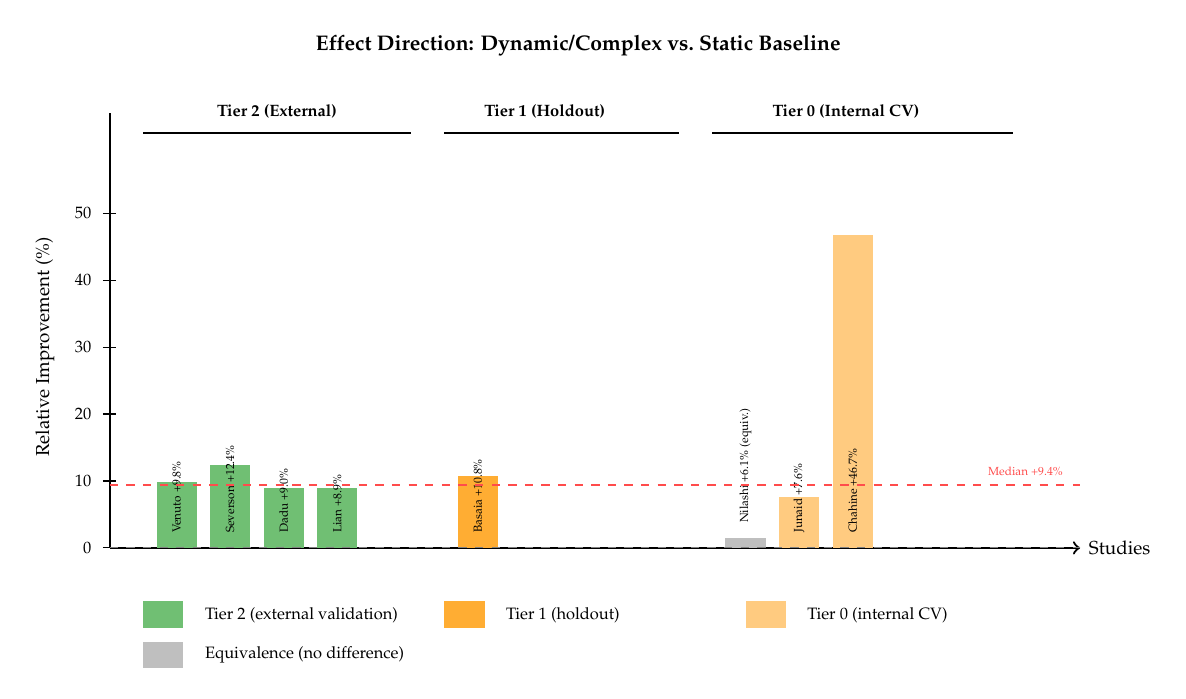
\begin{tikzpicture}[scale=0.85, transform shape]

% Title
\node[font=\small\bfseries] at (7, 7.5) {Effect Direction: Dynamic/Complex vs.\ Static Baseline};

% Axes
\draw[thick, ->] (0, 0) -- (14.5, 0) node[right, font=\footnotesize] {Studies};
\draw[thick] (0, 0) -- (0, 6.5);

% Y-axis labels
\node[font=\footnotesize, rotate=90, anchor=south] at (-0.7, 3) {Relative Improvement (\%)};
\foreach \y/\lab in {0/0, 1/10, 2/20, 3/30, 4/40, 5/50} {
    \draw (-0.1, \y) -- (0.1, \y);
    \node[font=\scriptsize, anchor=east] at (-0.15, \y) {\lab};
}

% Tier 2 (External Validation) - Green bars
\node[font=\scriptsize\bfseries, anchor=south] at (2.5, 6.3) {Tier 2 (External)};
\draw[thick] (0.5, 6.2) -- (4.5, 6.2);

\fill[lowrisk!80] (0.7, 0) rectangle (1.3, 0.98);
\node[font=\tiny, rotate=90, anchor=west] at (1.0, 0.1) {Venuto +9.8\%};

\fill[lowrisk!80] (1.5, 0) rectangle (2.1, 1.24);
\node[font=\tiny, rotate=90, anchor=west] at (1.8, 0.1) {Severson +12.4\%};

\fill[lowrisk!80] (2.3, 0) rectangle (2.9, 0.90);
\node[font=\tiny, rotate=90, anchor=west] at (2.6, 0.1) {Dadu +9.0\%};

\fill[lowrisk!80] (3.1, 0) rectangle (3.7, 0.89);
\node[font=\tiny, rotate=90, anchor=west] at (3.4, 0.1) {Lian +8.9\%};

% Tier 1 (Holdout) - Orange bars
\node[font=\scriptsize\bfseries, anchor=south] at (6.5, 6.3) {Tier 1 (Holdout)};
\draw[thick] (5.0, 6.2) -- (8.5, 6.2);

\fill[modrisk!80] (5.2, 0) rectangle (5.8, 1.08);
\node[font=\tiny, rotate=90, anchor=west] at (5.5, 0.1) {Basaia +10.8\%};

% Tier 0 (Internal CV) - Yellow/light bars
\node[font=\scriptsize\bfseries, anchor=south] at (11, 6.3) {Tier 0 (Internal CV)};
\draw[thick] (9.0, 6.2) -- (13.5, 6.2);

\fill[gray!50] (9.2, 0) rectangle (9.8, 0.15);
\node[font=\tiny, rotate=90, anchor=west] at (9.5, 0.25) {Nilashi +6.1\% (equiv.)};

\fill[modrisk!50] (10.0, 0) rectangle (10.6, 0.76);
\node[font=\tiny, rotate=90, anchor=west] at (10.3, 0.1) {Junaid +7.6\%};

\fill[modrisk!50] (10.8, 0) rectangle (11.4, 4.67);
\node[font=\tiny, rotate=90, anchor=west] at (11.1, 0.1) {Chahine +46.7\%};

% Reference line at 0
\draw[dashed, gray] (0, 0) -- (14.5, 0);

% Median line
\draw[dashed, red!70, thick] (0, 0.94) -- (14.5, 0.94);
\node[font=\tiny, red!70, anchor=west] at (13.0, 1.15) {Median +9.4\%};

% Legend
\fill[lowrisk!80] (0.5, -1.2) rectangle (1.1, -0.8);
\node[font=\scriptsize, anchor=west] at (1.3, -1.0) {Tier 2 (external validation)};
\fill[modrisk!80] (5.0, -1.2) rectangle (5.6, -0.8);
\node[font=\scriptsize, anchor=west] at (5.8, -1.0) {Tier 1 (holdout)};
\fill[modrisk!50] (9.5, -1.2) rectangle (10.1, -0.8);
\node[font=\scriptsize, anchor=west] at (10.3, -1.0) {Tier 0 (internal CV)};
\fill[gray!50] (0.5, -1.8) rectangle (1.1, -1.4);
\node[font=\scriptsize, anchor=west] at (1.3, -1.6) {Equivalence (no difference)};

\end{tikzpicture}
\caption{\textbf{Harvest plot of comparative effectiveness by validation tier.} Each bar represents one head-to-head comparison study ($n=8$). Bar height corresponds to the relative improvement of the dynamic/complex model over the static baseline. Studies are stratified by validation tier: Tier~2 (external, green), Tier~1 (holdout, orange), Tier~0 (internal CV, light orange). The dashed red line indicates the median relative improvement ($+9.4\%$). Seven of eight comparisons (87.5\%) favoured the dynamic model; one showed equivalence (Nilashi 2022); none favoured the static baseline. Externally validated studies (Tier 2) showed a median $+9.2\%$ improvement, while internally validated studies (Tier 0) showed $+6.8\%$, suggesting that internal validation may modestly overestimate or that higher-quality studies exhibit larger gains.}
\label{fig:s2_harvest}
\end{figure}

\end{document}
